\documentclass[AutoFakeBold]{tstextbook}
\usepackage{xeCJK}
\usepackage{ctex}
\usepackage{fontspec}
\usepackage{hyperref,amsmath,mhchem,cancel,braket}
\usepackage{physics2}
\hypersetup{hidelinks}
\usepackage{esdiff} 
\usepackage{subfigure}
\setCJKmainfont{NSimSun}
\setmainfont{Segoe UI}
\bibliographystyle{plain}
\usepackage{natbib}
\usepackage{unicode-math}
\newcommand{\bd}[1]{\symbfit{#1}}
\newcommand{\di}{\mathrm{d}}
\newcommand{\arr}{
	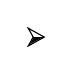
\begin{tikzpicture}
		\draw[white,fill=black] (0,0)--(.4em,0)--(-.18em,-.32em)--(0,0); %下方三角填充
		\draw (0,0)--(-.18em,-.32em)--(.4em,0)--(-.18em,.32em)--(0,0); %边缘轮廓
		\draw (0,0)--(.4em,0); %中间那条横线
	\end{tikzpicture}}
\tcbuselibrary{breakable}
\definecolor{ztxgreen}{RGB}{0, 120, 80}
\newtcolorbox{pointlist}[2][]{colframe=blue!65!green,colback=white,fonttitle=\bfseries\large\kaishu,fontupper=\kaishu,breakable,title=#2,#1}
\newtcolorbox{examplelist}{colframe=green!40!yellow!50!blue,colback=white!95!black,fontupper=\fangsong,breakable}
\newtcolorbox{solution}{before upper={\textit{\bfseries 解}:},colframe=white,colback=white!95!black!95!green,fontupper=\kaishu,breakable}
\newtcolorbox[auto counter, number within=chapter,list type=subsubsection, list inside=toc]{refquestion}{before lower={{\bfseries Answer}:},colframe=green!60!red!60!blue,colback=white!95!black!,fontupper=\kaishu,fontlower=\kaishu,breakable,title={\bfseries{\large{\fangsong 思考题 \thetcbcounter}}}}
\newtcolorbox[auto counter, number within=chapter,list type=subsubsection, list inside=toc]{Dedis}{colframe=ztxgreen,colback=white,fontupper=\kaishu,fontlower=\kaishu,breakable,title={\bfseries{\large{ Detailed Discussion \thetcbcounter}}}}
\newcommand \dbar {\text{đ}}


\numberwithin{equation}{section}
\begin{document}

\tsbook{\songti 统计力学笔记}
{\large \kaishu 陶洋 \ 杨春雨\\
    千淘万漉虽辛苦,淘尽黄沙始到金。}
{Ts\TeX tbook}
{2023}
{20603}{206--03--2023--01--1}{1.0}
{USTC}
{Hefei}





%---------------------------------------------------------------------------
% Chapters
%---------------------------------------------------------------------------
\frontmatter
\chapter*{前言} % (fold)
\label{cha:前言}

这个笔记的主体部分由2019级陶洋学长完成,我拿到陶洋学长的笔记之后,结合自己在23年春统计力学课程的一些笔记,将其转换成了\LaTeX 代码。结合台湾新竹清华大学林秀豪教授的课程,补充了一点比如玻尔兹曼方程、半导体和相变的朗道唯象理论等我觉得既有用又有趣的内容,同时依据我自己所学方向,增补了一些非平衡态热力学和基于统计力学的分子动力学模拟的概述。

由于我们能力有限(特别是我增补的部分并不是老师上课讲授的内容),不当之处在所难免,如果有任何错误或者不当之处,欢迎通过邮件(\href{mailto:chunyuyang@ustc.edu}{chunyuyang@ustc.edu})联系我指出,感谢每一份真诚的建议。

完成这份笔记的过程中,许多人指出了我的问题或者与我分享了他们的理解,他们是20级化院彭子骏、王怀宇、禤科材。



\begin{flushright}
    
\includegraphics[width=0.24\textwidth]{images/signature.png}\\
    2023年3月于中国科大 
\end{flushright}

% chapter 前言 (end)


%---------------------------------------------------------------------------
\mainmatter
%---------------------------------------------------------------------------

\chapter{导言和系综理论基础} % (fold)
\label{cha:导言和系综理论基础}
\section{导言} % (fold)
\label{sec:导言}
\subsection{概述}
统计力学的研究的是由大量的微观粒子组成的宏观系统的宏观物理性质。这些物理性质包括熵$S$、温度$T$、内能$U$、压强$p$、体积$V$、自由能$F$,粒子数$N$、化学势$\mu$、热容$C_V$。\textbf{它们并不是独立的而是相互依赖的}。

接下来中我们会看到,在过去的几个世纪中我们发现的规律,比如理想气体的波义耳定律和查理定律,黑体辐射的维恩位移定律,磁性物质的居里定律。这些定律都不是基本的,有时候我们只需要用经典力学再加上一点统计力学的研究方法,就可以导出这些结果,有的时候经典物理是不够的,我们还需要借助一点点量子力学的知识。


在统计力学这门课程中,我们一般研究的是热力学平衡态\index{热力学平衡态},也被称为状态。一个系统的热力学状态由宏观性质确定,也由宏观性质描述。确定一个单组分均相系统的状态至少需要三个宏观性质,这三个宏观性质中至少需要一个广度量。这三个量被我们称为状态参量\index{状态参量}。

统计力学的研究方法和前面的经典物理是不同的,比如,我们对于一个粒子是没有办法定义温度的,但是如果没有温度,我们去理解现实世界。同时,我们也不可能用研究单个粒子的方法(写出体系的薛定谔方程,求解其本征态)来研究统计力学系统,不仅对多达$10^{23}$量级的粒子是不可能的,即使是对23个粒子,这也是非常困难的事情。所以统计力学不研究微观性质,但是是从微观态出发用统计学方法得到系统的宏观性质。

\subsection{遍历性假设}
\begin{theorem}[遍历性假设\index{遍历性假设}]
       在一个宏观测量的时间内,宏观系统以一定概率遍历了所有可能的微观态。测量的结果正是历经各态的平均。
\end{theorem}
% section 导言 (end)
\section{系综理论基础} % (fold)
\label{sec:系综理论基础}
\subsection{概述} % (fold)
\label{sub:概述}
我们常常讨论的系综\index{系综}主要有微正则系综、正则系综、巨正则系综和恒温恒压系综,其中巨正则系综和恒温恒压系综被统称为广义系综。\textbf{系综本质上是一种研究宏观系统的理论方法},宏观系统的性质不会因为系统的研究方法不同而不同。

对于微正则系综,我们同时固定了系统的体积$V$,能量$E$,粒子数$N$,因此没有能量或者粒子的交换,也就是说,微正则系综是一群孤立系统的集合。

对于正则系综,我们选取的状态参数为系统的体积$V$,粒子数$N$,温度$T$,相比较于微正则系综,正则系综能够发生能量交换但是不会存在物质交换。所以正则系综是一群达到了热平衡的孤立系统的集合。

巨正则系综的状态参数为系统的化学势$\mu$,体积$V$,温度$T$,因此巨正则系综既可以发生能量交换也可以发生物质交换。所以巨正则系综是一群达到了粒子数平衡和热平衡的开放系统的集合。

等温等压系综的状态参量为系统的粒子数$N$,压强$p$,温度$T$,等温等压系综可以发生能量交换,同时体积也能够发生变化,因此是一个达到压强和热平衡的封闭系统。

将微正则系综的一个或者两个状态广延(extensive)量\index{广延量}转变成其所对应的强度(intensive)量\index{强度量},我们就得到了后面三个系综。

\begin{example}
       我们能不能以$\mu,p,T$作为状态参量?
\end{example}
\begin{solution}
       我们知道$\di E= \mu \di N -p \di V +T\di S$,又考虑到$E=\mu N -pV+TS$,所以$N\di \mu -V\di p +S\di T=0$,因此$\mu,p,T$并不是独立的。
\end{solution}

接下来我们当然可以问,是否可以将微正则系综中的状态参量中的$V$或者$N$替换掉而保持其余两个不变(或者两个都换掉仅保持$E$不变),对于实际存在的系统,这是不能够发生的。所以,\textbf{有且仅有我们上述讨论的四种系综}。

系综理论只是获得系统宏观热力学性质的一种方法,我们将在稍后不断发现,系综理论和我们最终获得的系统的热力学关系不存在联系。
% subsection 概述 (end)
\subsection{微正则系综} % (fold)
\label{sub:微正则系综}

微正则系综的状态参量为$(N,V,E)$,于是系统的微观状态数也是$N,V,E$的函数。假设系统的总微观状态数为$\Omega(N,V,E)$,那么系统的任意一个微观态的概率为\begin{equation}
       p=\frac{1}{\Omega}
\end{equation}
这个结论是统计力学中最基本的假设,我们称之为\textbf{等概率原理}\index{等概率原理}。

因为\begin{equation}
       \di E= T\di S-p\di V +\mu \di N
\end{equation}
所以\begin{equation}
       \di S =\frac{1}{T} \di E + \frac{p}{T}\di V -\frac{\mu}{T}\di N
\end{equation}
而由Boltzman公式\index{玻尔兹曼公式}:
\begin{equation}
       S=k\ln \Omega
\end{equation}
所以就有\begin{equation}
       \di \ln \Omega =\beta \di E +\beta p\di V -\beta \mu \di N
\end{equation}
其中$\displaystyle \beta=\frac{1}{k T}$。

因此\begin{equation}
       \beta=\diffp*{\ln \Omega}{E}{{V,N}},\quad p=\frac{1}{\beta} \diffp*{\ln\Omega}{V}{{E,N}},\quad \mu =-\frac{1}{\beta} \diffp*{\ln \Omega}{N}{{E,V}}
\end{equation}
为了简化符号,我们将$\sigma=\ln \Omega$定义为fundamental entropy。

但是将系统的状态完全固定在$(N,V,E)$显然是不物理的,因此我们说的能量为$E$应该事实上是能量介于$E\sim E+\di E$。进而我们引入“累计分布函数\index{累计分布函数}”和“态密度函数\index{态密度函数}”:
\begin{definition}
       能量处于$0\sim E$的微观态的总数为$\Phi (E)$,我们称之为累积分布函数。
\end{definition}
\begin{definition}
       对累积分布函数求导数可以得到态密度\begin{equation}
              \overline{\Omega}(E)=\Phi'(E)
       \end{equation}
       其对应于处于$E\sim E+\di E$之间的微观态数量
       \begin{equation}
              \Omega(E)=\overline{\Omega}(E)\di E
       \end{equation}
\end{definition}

\begin{example}
       考虑一个三维势箱中的粒子,三维势箱的长宽高都是$a$。

       由量子力学结论我们知道,系统的能量为\begin{equation}
              \varepsilon_{n_x,n_y,n_z}=\frac{h^2}{8 ma^2} (n_x^2+n_y^2+n_z^2),\quad n_x,n_y,n_z=1,2,3,...
       \end{equation}
       考虑三维空间中的任意一个点$(n_x,n_y,n_z)$,其总是会对应于一个$x,y,z$分别位于$(n_x-1,n_x),(n_y-1,n_y),(n_z-1,n_z)$之间的一个立方体,这样的立方体数量就对应了微观态的数量。因此,考虑能量介于$0\sim E$之间的微观态数量,其数值上就应该近似等于半径为$\displaystyle \sqrt{\frac{8ma^2 E}{h^2}}$的球体位于第一象限内的体积,于是\begin{equation}
              \Phi(E)=\frac{4}{3}\pi R^3 \times\frac{1}{8}=\frac{\pi}{6}\left(\frac{8ma^2 E}{h^2}\right)^{3/2}
       \end{equation}
       进而就有系统的态密度为\begin{equation}
              \overline{\Omega}(E)=\frac{\pi}{4}\left(\frac{8ma^2 }{h^2}\right)^{3/2}E^{1/2}
       \end{equation}

       单个粒子的能量大约在$kT\sim10^{-20}$的量级,质量约为$10^{-26}\mathrm{kg}$量级。于是$\displaystyle \frac{h^2}{8ma^2}\sim 10^{-42}$,不妨设$\displaystyle \frac{\di E}{E}\sim 10^{-3}$,于是态密度大约在\begin{equation}
              \Omega(E)=\frac{\pi}{4}\left(\frac{8ma^2 }{h^2}\right)^{3/2}E^{3/2}\cdot \frac{\di E}{E}\sim 10^{42\times \frac{3}{2}-20\times 3/2- 3} =10^{30}
       \end{equation}
       这是一个非常巨大的数字。
\end{example}

上述结果可以非常自然地推广到$N$个无相互作用的粒子的体系,$3N$维球体的体积公式(证明见\ref{sec:N维球体的体积和表面积})为
\begin{equation}
       V_{3N}(R)=\frac{\pi^{3N/2}R^{3N}}{\Gamma (\frac{3N}{2}+1)}
\end{equation}
进而\begin{equation}
       \Phi(E)=\frac{1}{2^{3N}} \frac{\pi^{3N/2}}{\Gamma(\frac{3N}{2}+1)} \left(\frac{8ma^2 E }{h^2}\right)^{3N/2} \times\frac{1}{N!}
\end{equation}
上述表达式中$1/2^{3N}$是来自于每一个维度只取其正的二分之一,$1/N!$则是来自粒子的全同性要求。

\begin{Dedis}
	为什么$1/N!$项就可以描述粒子的全同性要求?
	\tcblower
	我们以三个粒子为例,当它们分别占据三个不同的状态的时候,则可能的排列数为$3!=6$,确实重复计算了$N!$次,但是假如有两个粒子占据同一个态,则实际上可能的排列只有三种,如果三个粒子占据同一个状态,则其排列数其实只有一种。但是理想气体是\textbf{稀薄}的,所以两个粒子占据同一个态的概率非常低,可以忽略。\textbf{理想气体的稀薄既指空间上占据的稀薄,也是态空间中分布的稀薄}。
\end{Dedis}


进而就有\begin{equation}
       \Omega(E)=\Phi'(E)\di E
\end{equation}

对$\Omega(E)$取对数,可以得到\begin{equation}
       \ln \Omega(E)=f(N)+(\frac{3}{2}N-1)E+N\ln V+\ln \frac{\di E}{E}
\end{equation}
其中$V=a^3$。又因为\begin{equation}
       \beta=\diffp*{\ln\Omega}{E}{N,V}=(\frac{3}{2}N-1)\frac{1}{E}
\end{equation}

\begin{remark}
我们将$\frac{\di E}{E}$看作常数。       
\end{remark}

考虑到$N$非常的大,于是$\displaystyle \beta\sim \frac{3}{2}N\frac{1}{E}$,所以就有\begin{equation}
       E=\frac{3}{2}NkT
\end{equation}
而\begin{equation}
       \diffp*{\ln\Omega}{V}{N,E}=\beta p=\frac{N}{V}
\end{equation}
这就得到了理想气体状态方程$pV=NkT$。
% subsection 微正则系综 (end)
\subsection{总结} % (fold)
\label{sub:1.3总结}
当我们研究微正则系综的时候,我们首先关心的是系统的multiplicity function $\Omega$,从此出发我们可以获得所有我们想要的物理量。现在我们对使用微正则系综研究问题的范式做一个总结。

\begin{pointlist}{微正则系综研究问题的范式}
       \begin{itemize}
              \item 首先明确系综的状态参量是$N,V,E$;
              \item 求出系统的multiplicity function $\Omega$;
              \item 将$\Omega$代入Boltzman公式$S=k_B \ln \Omega$,进而代入其他热力学基本关系,得到状态数和其他热力学量的关系;
              \item 结合微正则系综的基本关系和热力学的一些结论,获得一些有意义的结论。
       \end{itemize}
\end{pointlist}
接下来我们看一道例题:
\begin{example}
       现在有一个由位于磁场$H$中的由$N$个无相互作用的自旋构成的系统,其能量满足\begin{equation}
              -\sum_{j=1}^N\mu_J H,\quad \mu_j =\pm \mu.
       \end{equation}
       尝试求这个系统的温度。
\end{example}
\begin{solution}
       设自旋朝上的数量为$N_\uparrow$,自选朝下的数量为$N_\downarrow$。spin excess定义为\begin{equation}
              2s=N_\uparrow-N_\downarrow
       \end{equation}
       于是系统的能量$E=-2s \mu H$。体系可能的微观状态数为\begin{equation}
              \Omega =C_{N}^{N_\uparrow}=\frac{N!}{N_\downarrow !N_\uparrow!}
       \end{equation}
       于是\begin{equation}
              \begin{aligned}
              \sigma&=\ln\Omega\propto N\ln N -N -(N_\downarrow \ln N_\downarrow -N\downarrow + N_\uparrow \ln N_\uparrow -N_\uparrow)\\
              &=\ln\Omega\propto N\ln N -N -(N_\downarrow \ln N_\downarrow + N_\uparrow \ln N_\uparrow)
              \end{aligned}
       \end{equation}
       因为$N_\uparrow+N_\downarrow=N$,所以\begin{equation}
              N_\uparrow=\frac{N}{2}+s,\quad N_{\downarrow}=\frac{N}{2}-s
       \end{equation}
       进而\begin{equation}
              \sigma=\ln\Omega\propto N\ln N -N -[(\frac{N}{2}-s) \ln (\frac{N}{2}-s) +(\frac{N}{2}+s) \ln(\frac{N}{2}+s)]
       \end{equation}
       我们称$\displaystyle \tau=\frac{1}{kT}$为fundamental temperature。于是\begin{equation}
              \tau=\diffp*{\sigma}{E}{N,V} = \diffp*{\sigma}{s}{N,V}\diff{s}{E}=\frac{1}{2\mu H}\ln \frac{N+2s}{N-2s}
       \end{equation}
	   于是当$s<0$的时候,系统的温度是一个负数。这和我们的认知产生了一些冲突。因为这里的系统是一个受限系统,从而在能量增长的过程中出现了熵减的现象。
\end{solution}

如果我们可以了解一个系统的multiplicity function,那么理论上我们就能够充分的了解这个系统。不过,在大多数时候,了解这个系统的multiplicity function是非常困难的。所以我们需要发展一些新的方法,这也就是我们后面将会讨论的内容。
\begin{refquestion}
       尝试求锂原子前五个能级的多重度。
\end{refquestion}
% subsection 总结 (end)
% section 系综理论基础 (end)
\section{Temperature} % (fold)
\label{sec:temperature}
温度在经典热力学和统计热力学中都应该是最基本的物理量之一,但是截止目前我们还没有对温度给出清晰的定义。

在物理学发展史上定义温度的热力学第零定律\index{热力学第零定律}也晚于热力学第一定律和第二定律,但是它是热力学第一定律和第二定律的基础,所以被称为第零定律。

\begin{law}[热力学第零定律]
       若两个热力学系统均与第三个系统处于热平衡状态,此两个系统也必互相处于热平衡。
\end{law}

接下来我们来具体看一下,为什么温度可以成为两个系统达成热平衡的标志?

系统的multiplicity function是能量的函数,因此\begin{equation}
       \Omega=\sum_{u_1} \Omega_1(U_1) \Omega_2(U_2),\quad U=U_1+U_2\  \text{is a constant}
\end{equation}

如图\ref{fig:temperature},两个系统相互接触,假设他们达成热平衡,那么我们知道系统应该处于最概然分布,即$\Omega=\Omega_{max}$。如果系统正处于最概然分布,那么就应该有\begin{equation}
       \di \Omega=\Omega_2 \di \Omega_1+\Omega_1 \di \Omega_2=0
\end{equation}
\begin{figure}[h]
       \centering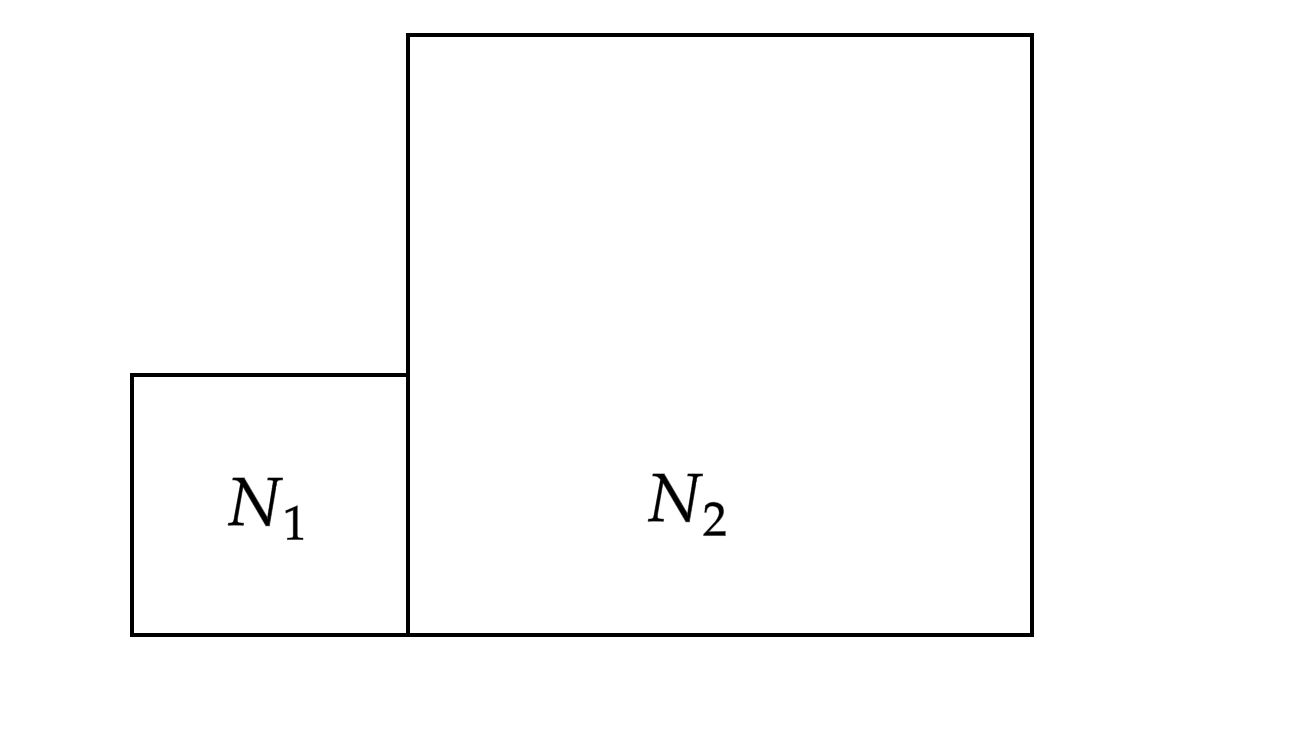
\includegraphics[width=0.5\textwidth]{fig/temperature.png}
       \caption{两个相互接触的热力学系统}
       \label{fig:temperature}
\end{figure}

因为\begin{equation}
       \di \Omega_1=\diffp*{{\Omega_1}}{{U_1}}{{N_1,V_1}}\di U_1 + \diffp*{{\Omega_1}}{{N_1}}{{U_1,V_1}}\cancelto{0}{\di N_1}+\diffp*{{\Omega_1}}{{V_1}}{{U_1,N_1}}\cancelto{0}{\di V_1}
\end{equation}
$\Omega_2$也是类似的,因此我们就有\begin{equation}
       \di \Omega=\Omega_1\diffp*{{\Omega_1}}{{U_1}}{{N_1,V_1}}\di U_1 + \Omega_2\diffp*{{\Omega_2}}{{U_2}}{{N_2,V_2}}\di U_2=0
\end{equation}
考虑到$U=U_1+U_2=\text{constant}$,因此$\di U_1+\di U_2=0$,所以\begin{equation}
       \di \Omega=\left(\Omega_2\diffp*{{\Omega_1}}{{U_1}}{{N_1,V_1}}- \Omega_1\diffp*{{\Omega_2}}{{U_2}}{{N_2,V_2}}\right)\di U_1=0
\end{equation}
从而
\begin{equation}
       \diffp*{{\ln \Omega_1}}{{U_1}}{{N_1,V_1}}- \diffp*{{\ln \Omega_2}}{{U_2}}{{N_2,V_2}}=0
\end{equation}
于是我们定义fundamental temperature $\tau =k_B T$满足\begin{equation}
       \frac{1}{\tau}=\diffp*{{\ln \Omega}}{{U}}{{N,V}}
\end{equation}
所以两个系统处于热平衡也就是\begin{equation}
       \tau_1=\tau_2
\end{equation}

从$\tau$的定义我们有\begin{equation}
       \Omega(U+\Delta U)=\Omega(U) e^{\frac{\Delta U}{\tau}}\quad\text{for}\ \Delta U\ \text{is small}
\end{equation}
于是当两个系统处于热平衡的时候,他们交换热量$\Delta U$\begin{equation}
       \Omega_1(U_1+\Delta U)\Omega_2(U_2-\Delta U)=\Omega_1(U_1) e^{\frac{\Delta U}{\tau}}\Omega(U_2)e^{-\frac{\Delta U}{\tau}}=\Omega_1(U_1)\Omega_2(U_2)
\end{equation}
这个关系要成立,$\Delta U$必须非常小。从这个关系我们可以发现温度可以表述成:系统的温度为$T$指的是,在平衡态附近当系统的能量增大一个$k_B T$的时候,系统的multiplicity function增大$e$倍。同时,因为$\Omega$依赖于$N,U,T$,所以只有对于平衡态才能够定义温度。



% section 温度 (end)
\begin{review}
     \item 遍历性假设
     \item 系综的基本概念
     \item 系统的状态参量
     \item 微正则系综及其应用
     \item mulltilicity function
     \item 温度的物理意义
\end{review}

\section{习题} % (fold)
\label{sec:习题1}
\begin{enumerate}
	\item Two systems, $A$ and $B$, of identical composition, are brought together and allowed to exchange both energy and particles, keeping volumes $V_A$ and $V_B$ constant. Show that the minimum value of the quantity $\left(\di  E_A / \di N_A\right)$ is given by
	$$
	\frac{\mu_A T_B-\mu_B T_A}{T_B-T_A}
	$$
	where the $\mu$ 's and the $T$ 's are the respective chemical potentials and temperatures.
	\item Making use of the fact that the entropy $S(N, V, E)$ of a thermodynamic system is an extensive quantity, show that
	$$
	N\left(\frac{\partial S}{\partial N}\right)_{V, E}+V\left(\frac{\partial S}{\partial V}\right)_{N, E}+E\left(\frac{\partial S}{\partial E}\right)_{N, V}=S .
	$$

	Note that this result implies that $(-N \mu+P V+E) / T=S$, that is, $N \mu=E+P V-T S$.

\end{enumerate}
% section 习题 (end)
% chapter 导言和系综理论基础 (end)
%---------------------------------------------------------------------------
%---------------------------------------------------------------------------
\chapter{正则系综和广义系综} % (fold)
\label{cha:正则系综和广义系综}
\section{正则系综} % (fold)
\label{sec:正则系综}
\subsection{正则系综和配分函数} % (fold)
\label{sub:正则系综和配分函数}
所谓正则系综,就是固定了$N,V,T$作为状态参量的系综。一般来说,我们可以将正则系综看作微正则系综的一个子系统。让正则系综与热库\index{热库}接触(reservoir)。当正则系综和环境达到热平衡的时候,两者就构成了一个微正则系综。
\begin{figure}[h]
       \centering
       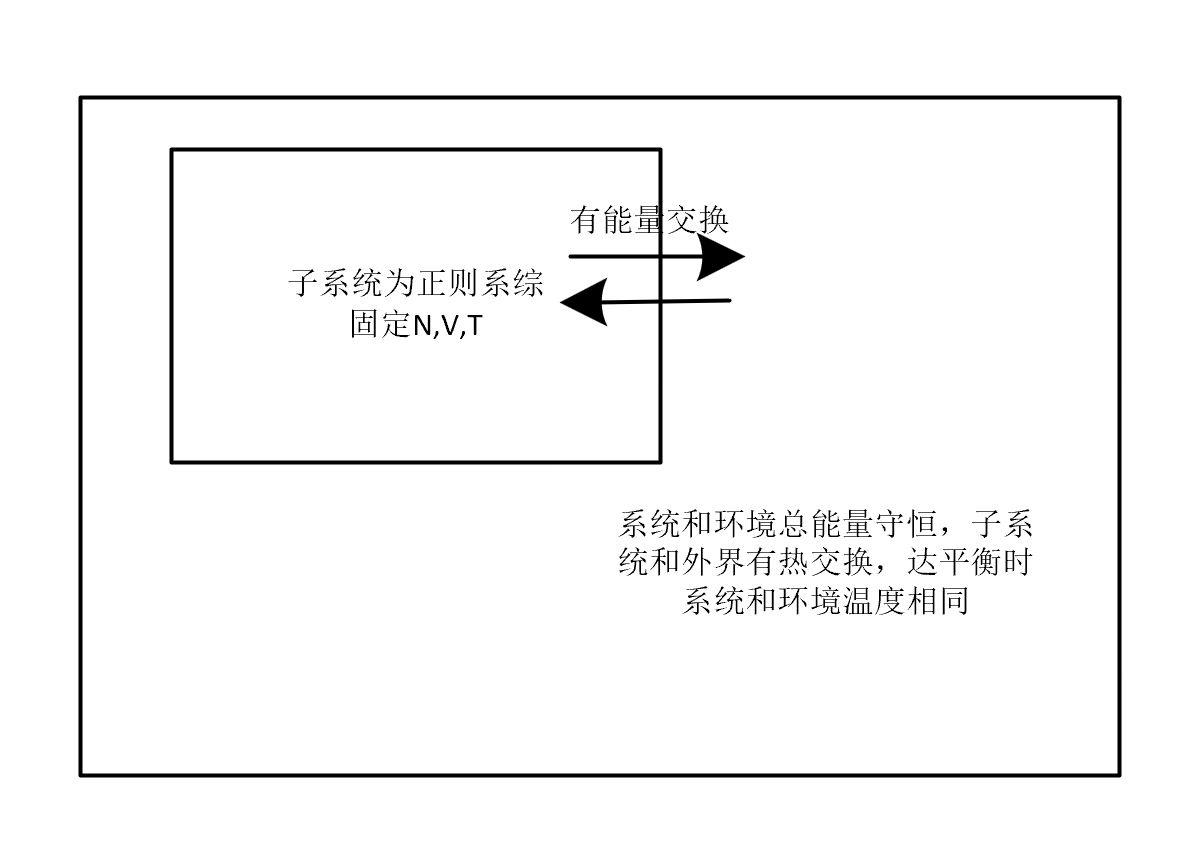
\includegraphics[width=0.45\textwidth]{fig/正则系综.png}
       \caption{正则系综}
\end{figure}

系统和环境的总能量是一个定值\begin{equation}
       E_{sys}+E_{envir}=E_0
\end{equation}
所以$E_{envir}=E_0-E_{sys}$,考虑系统处于能量$E_{sys}$时的概率,显然,应该正比于这个时刻系统和环境的状态数之积
\begin{equation}
       p(E_{sys})\propto \Omega_{sys}(E_{sys})\Omega(E_{0}-E_{sys})
\end{equation}
我们可以直接考虑系统处于某一个状态的概率,于是\begin{equation}
\begin{aligned}
       p(E_{sys})&\propto \Omega(E_{0}-E_{sys})\\
       &=e^{\ln \Omega(E_{0}-E_{sys})}
\end{aligned}
\end{equation}
假设$E_0\ll E_{sys}$,因此
\begin{equation}
       \ln \Omega(E_{0}-E_{sys})=\ln \Omega(E_0)-E_{sys} \left.\diffp{\Omega}{E}\right|_{E=E_0}
\end{equation}
\begin{definition}
       定义\begin{equation}
              \beta=\left.\diffp{\Omega}{E}\right|_{E=E_0}
       \end{equation}
\end{definition}
因为对于微正则系综$E_0$是一个常数,因此$\Omega(E_0)$也是一个常数,所以\begin{equation}
       p\propto e^{-\beta E_{sys}}
\end{equation}
归一化之后可以得到\begin{equation}
       p_i =\frac{\displaystyle e^{-\beta E_{sys}}}{\displaystyle \sum e^{-\beta E_{sys}}}
\end{equation}其中,求和是对所有可能的状态求和。

\begin{definition}
       我们记\begin{equation}
              Q=\sum e^{-\beta E_{sys}(N,V)}=Q(N,V,T)
       \end{equation}
       为系统的配分函数\index{配分函数}。
\end{definition}

当然,对系统的所有状态的求和也可以变换成对能级的求和\begin{equation}
      \begin{aligned}
       Q&=\sum e^{-\beta E_{sys}(N,V)}=\sum_{E}\Omega(E) e^{-\beta E}\\
       &=\int_0^{+\infty} \overline{\Omega}(E) e^{-\beta E} \di E 
      \end{aligned} 
\end{equation}
从上式我们不难发现正则配分函数就是对微正则系综中的态密度函数做了一个Laplace变换,这也反映了两者的等价性。
% subsection 正则系综和配分函数 (end)
\subsection{均值、涨落和能量的正则分布} % (fold)
\label{sub:均值、涨落和能量的正则分布}
首先我们来考虑能量的均值\index{均值}
\begin{equation}
\begin{aligned}
       \braket{E}&=\sum_{v}p_v E_v =\sum_{v}\frac{e^{-\beta E_v}E_v}{Q}\\
       &=-\diffp*{\ln Q}{\beta}{N,V}\label{equ:energy mean in canolical ensemble}
\end{aligned}
\end{equation}

然后我们就可以来考虑能量的涨落\index{涨落}
\begin{equation}
       \braket{(\Delta E)^2}=\braket{E^2}-\braket{E}^2
\end{equation}
对于$\braket{E^2}$,我们有\begin{equation}
\begin{aligned}
       \braket{E^2}&=\sum_{v}p_v E_v^2 =\sum_{v}\frac{e^{-\beta E_v}E_v^2}{Q}\\
       &=\frac{1}{Q} \diffp[2]{Q}{\beta}\\
\end{aligned}
\end{equation}
因此\begin{equation}
       \begin{aligned}
              \Delta ^2 &=\braket{E^2}-\braket{E}^2=\frac{1}{Q} \diffp[2]{Q}{\beta}-\frac{1}{Q^2} \left(\diffp[1]{Q}{\beta}\right)^2\\
       &=\diffp{}{\beta} \left(\frac{1}{Q} \diffp{Q}{{\beta}}\right)\\
       &=-\diffp{{\braket{E}}}{\beta}
       \end{aligned}
\end{equation}

\begin{remark}
       一个有用的微分关系:\begin{equation}
              \diffp{}{\beta} =\diffp{}{T} \diffp{T}{\beta}=-kT^2 \diffp{}{T}
       \end{equation}
\end{remark}

因此就有了\begin{equation}
              \braket{(\Delta E)^2} =\diffp{{\braket{E}}}{\beta}=kT^2 \diffp{\braket{E}}{T} =kT^2 C_V
\end{equation}

\begin{definition}
       定义涨落的相对值\index{相对涨落}为\begin{equation}
              \sigma_E=\frac{\sqrt{\braket{(\Delta E)^2}}}{\braket{E}}=\frac{\sqrt{kT^2C_V}}{\braket{E}}\sim O(\frac{1}{\sqrt{N}})
       \end{equation}
\end{definition}
\begin{remark}
       这里的$C_V$和$\braket{E}$都是广延量与$N$成线性关系。
\end{remark}

这个结果表明,当$N$很大的时候,能量的涨落非常小的,于是在平衡时,正则系综趋于零的能量涨落并不和微正则系综固定的能量相矛盾。

我们知道系统处于某一个特定的能级的概率为\begin{equation}
       p(E)=\frac{e^{-\beta E}}{Q} \Omega(E)
\end{equation}
所以\begin{equation}
       \ln p(E)=\ln \Omega(E)-\beta E-\ln Q
\end{equation}
现在我们关心的是它在$\braket{E}$附近的分布,于是我们对他做Taylor展开\begin{equation}
       \ln p(E)=\ln p(\braket{E})+\left.\diffp{\ln p}{E}\right|_{E=\braket{E}}(E-\braket{E})+\frac{1}{2}\left.\diffp[2]{\ln p}{E}\right|_{E=\braket{E}}(E-\braket{E})^2+\cdots
\end{equation}

\begin{remark}
       我们通常写的热力学关系式中的热力学量实际上都是他们的均值,实际上\begin{equation}
              \diffp*{\ln(\Omega(E))}{E}{N,V}\neq \beta.
       \end{equation}
       而是\begin{equation}
             \left. \diffp*{\ln(\Omega(E))}{E}{N,V}\right|_{E=\braket{E}}= \beta.
       \end{equation}
\end{remark}

我们有\begin{equation}
     \left.  \diffp{\ln p}{E}\right|_{E=\braket{E}} =\left. \diffp*{\ln(\Omega(E))}{E}{N,V}\right|_{E=\braket{E}}-\beta=0
\end{equation}
与此同时\begin{equation}
       \left. \diffp[2]{\ln p}{E}\right|_{E=\braket{E}}=\left. \diffp[2]{\ln(\Omega(E))}{E}\right|_{E=\braket{E}}=\diffp{\beta}{{\braket{E}}}=-\frac{1}{\braket{(\Delta E)^2}}< 0
\end{equation}
所以$E=\braket{E}$时$p(E)$取极大值,于是我们有\begin{equation}
       \ln p(E)=\ln p(\braket{E})-\frac{1}{2}\frac{1}{\braket{(\Delta E)^2}}(E-\braket{E})^2+O(E^2)
\end{equation}
也即\begin{equation}
       p(E)=p(\braket{E})\exp\left(-\frac{1}{2\braket{(\Delta E)^2}}(E-\braket{E})^2\right)
\end{equation}
$p(E)$形式上满足高斯分布,我们可以做一个简单的估算,$N\sim 10^{22}$,$\sigma_E\sim 10^{-11}$,$\displaystyle \left|\frac{\delta E}{\braket{E}}\right|\sim 10^{-10}$
于是就有\begin{equation}
       \frac{p(E)}{p(\braket{E})}=e^{-\frac{1}{2} \frac{10^{-20}}{10^{-22}}}=e^{-50}\sim 10^{-22}
\end{equation}
所以这个分布实际上非常地尖锐,接近$\delta(\braket{E})$。也就有\begin{equation}
       Q=\sum \omega(E) e^{-\beta E}\sim \omega(\braket{E}) e^{-\beta \braket{E}}
\end{equation}
% subsection 均值、涨落和能量的正则分布 (end)
\subsection{其他热力学关系} % (fold)
\label{sub:其他热力学关系}
回顾我们的热力学基本关系式,我们有\begin{equation}
       \di E =T \di S -P \di V +\mu \di N
\end{equation}
对$E$做一个勒让德变换,我们可以得到Helmholtz自由能\index{Helmholtz自由能}\begin{definition}[Helmholtz自由能]
       \begin{equation}
              A=E-TS
       \end{equation}
\end{definition}
我们可以得到\begin{equation}
       \di A =\di E -S\di T-T \di S =\mu \di N -P \di V -T \di S
\end{equation}
所以就有\begin{equation}
       S=-\diffp*{A}{T}{V,N}
\end{equation}
由Gibbs-Helmholtz关系\index{Gibbs-Helmholtz关系}\begin{equation}
\begin{aligned}
       \left(\diffp{}{T} \frac{A}{T}\right)_{N,V}&=\frac{1}{T}\diffp{A}{T}-\frac{A}{T^2}       \\
       &=-\frac{S}{T}-\frac{E-TS}{T^2}=-\frac{E}{T^2}
\end{aligned}\end{equation}
回顾前面提到的数学关系\begin{equation}
       \diffp{}{T}=-\frac{1}{kT^2} \diffp{}{\beta}
\end{equation}
于是我们有\begin{equation}
       \diffp{{(\beta A)}}{\beta} =E 
\end{equation}
回顾正则系综中的结论\begin{equation}
       \braket{E}=-\diffp*{\ln Q}{\beta}{N,V}
\end{equation}
因此\begin{equation}
       \diffp{{(\beta A)}}{\beta}=-\diffp*{\ln Q}{\beta}{N,V}
\end{equation}
所以$\beta A$和$-\ln Q$只能相差一个关于$N,V$的常数,于是我们有\begin{equation}
       A=-kT\ln Q +kT f(N,V)
\end{equation}
我们考虑$T\to 0$的情形,于是我们有\begin{equation}
      \lim_{T\to 0} A=\lim_{T\to 0} E-TS=E_0 -k_B T\log \Omega(E_0)
\end{equation}
这个时候的配分函数\begin{equation}
       Q=\Omega(E_0) e^{-\beta E_0}+\Omega(E_1)e^{-\beta E_1}+\cdots
\end{equation}
当$T\to 0$的时候,$e^{-\beta E_1}$会远远小于$e^{-\beta E_0}$,于是我们有\begin{equation}
       \lim_{T\to 0} A=-kT\ln Q+kT f(N,V)=E_0 -kT\log \Omega(E_0) +kT f(N,V)
\end{equation}
与上式对比可知$f(N,V)=0$,这个结果对任意的$N,V$都应该成立,因此$f(N,V)\equiv 0$\footnote{老师课上讲的是取只有一个能级的情形来讨论。这和我们写的方法其实是等价的。}。于是我们有\begin{equation}
       A=-kT\ln Q
\end{equation}

从而\begin{equation}
       S=-\diffp*{A}{T}{N,V}=k\ln Q +k T \diffp*{\ln Q}{T}{N,V}=k\ln Q -\frac{1}{T}\diffp*{\ln Q}{\beta}{N,V}
\end{equation}
结合正则系综的结论\ref{equ:energy mean in canolical ensemble},我们就可以得到\begin{equation}
       S=k\ln Q +\frac{\braket{E}}{T}
\end{equation}
所以对于热力学极限情形就有\begin{equation}
       Q=\Omega(\braket{E}) e^{-\beta \braket{E}}
\end{equation}
即\begin{equation}
       A=-kT\ln Q =-kT\left(\ln \Omega(\braket{E}) +\beta \braket{E}\right)=E-TS
\end{equation}
这就又回到了我们最初的定义,这表明我们的理论是自洽的。

再结合我们的热力学基本公式\begin{equation}
       \di A=-S\di T-p\di V+\mu \di N-kT \di \ln Q -k \ln Q \di T
\end{equation}
移项整理后可以得到\begin{equation}
       \ln Q=\beta \left[(S-k\ln Q)\di T +p\di V -\mu \di N\right]
\end{equation}
即有\begin{equation}
       \diffp*{\ln Q}{T}{V,N}=\beta (S-k\ln Q),\quad \diffp*{\ln Q}{V}{T,N}=-\beta p,\quad \diffp*{\ln Q}{N}{T,V}=\beta \mu 
\end{equation}
到目前为止,正则系综配分函数与宏观热力学量之间的主要关系均已导出。
% subsection 其他热力学关系 (end)
\subsection{Gibbs熵公式} % (fold)
\label{sub:Gibbs熵公式}
前面我们提到的Boltzman公式$S=k_B\ln \Omega$是熵的一种表述形式,这种表述形式一般只对平衡态有效。熵还有另外一种更加普适的表述——Gibbs熵\begin{definition}[Gibbs熵]
       \begin{equation}
              S=-k\sum_v p_v \ln p_v
       \end{equation}
\end{definition}

\begin{remark}
      1. 这个结果看起来有点像$\ln p_v$的系综平均,不过当然不存在$S_v=-k\ln p_v$,因为熵建立在大量统计的基础上,单个微观态不能够有熵。

      \noindent 2.这个结果其实来自于Shannon Entropy。
\end{remark}

我们可以看到,对于我们之前讨论的微正则系综和正则系综,Gibbs熵和Boltzman熵是等价的。对于微正则系综,我们有\begin{equation}
       S=-k\sum_v p_v \ln p_v=-k\sum_{i=1}^\Omega \frac{1}{\Omega}\ln \frac{1}{\Omega}= k\ln \Omega
\end{equation}
对于正则系综,则有\begin{equation}
\begin{aligned}
       S&=-k \sum_v p_v \ln p_v=-k\sum_v \frac{e^{-\beta E_v}}{Q}\ln\left(\frac{e^{-\beta E_v}}{Q}\right)\\
       &=-k\sum_v \frac{e^{-\beta E_v}}{Q}\left(-\beta E_v -\ln Q\right)\\
       &=k\ln Q+\frac{\braket{E}}{T}
\end{aligned}
\end{equation}
% subsection Gibbs熵公式 (end)

\subsection{总结} % (fold)
\label{sub:2.1总结}
相比于微正则系综,正则系综的能量变成了一个变量,因此我们可以比较方便的讨论有关能量的问题。我们现在对正则系综的研究范式做一个总结。
\begin{pointlist}{正则系综的研究范式}
       \begin{enumerate}
              \item 明确系统的状态参量为$N,V,T$;
              \item 构建一个系统和环境的总体微正则系综,将系统作为对环境的微扰得到任意一个微观态的概率$\displaystyle p_v\propto e^{-\beta E_v}$,并引入正则配分函数\begin{equation}
                     Q=\sum_v e^{-\beta E_v}=\sum_E \Omega(E) e^{-\beta E}
              \end{equation}
              \item 从使用配分函数表达的概率触发,导出有关能量的均值、方差以及概率分布等基本规律;
              \item 引入$A=E-TS$,结合热力学关系进一步推出$S,p,\mu$等其他宏观热力学量。
       \end{enumerate}
\end{pointlist}
% subsection 总结 (end)

\begin{example}
       假设一个长宽高均为$L$的立方体中有$N$个理想气体分子,尝试求这个体系的熵。
\end{example}
\begin{solution}
       如果两个系统之间的相互作用很弱,那么它们的总能量近似满足\begin{equation}
              \varepsilon=\varepsilon_1+\varepsilon_2
       \end{equation}
       
       对于配分函数$Z$,我们就有\begin{equation}
       \begin{aligned}
              Z&=\sum_s e^{-\varepsilon_s/\tau}\\
              &=\sum_{s_1}\sum_{s_2}e^{-\varepsilon_{s_1}/\tau}e^{-\varepsilon_{s_2}/\tau}\\
              &=\sum_{s_1}e^{-\varepsilon_{s_1}/\tau}\sum_{s_2}e^{-\varepsilon_{s_2}/\tau}\\
              &=Z_1Z_2
       \end{aligned}
       \end{equation}
       这个结论可以直接推广到多个弱相互作用的系统的组合,于是对于一个粒子数为$N$的理想气体系统就有
       \begin{equation}
              Z_N=Z_1^N
       \end{equation}
       因此,只要了解了一个粒子的配分函数,就可以了解这个系统的配分函数,而理想气体中的一个粒子可以看作三维势箱中的粒子,因此就有\begin{equation}
              \varepsilon=\frac{\hbar^2 k^2}{2m}=\frac{\hbar^2 \pi^2}{2mL^2}(n_x^2+n_y^2+n_z^2)
       \end{equation}
       于是配分函数$Z_1$就满足\begin{equation}
              Z_1=\sum_n \exp({-\frac{\hbar^2 \pi^2 n^2}{2m\tau L^2}})=\left[\sum_{n_x} \exp(-\frac{\hbar^2 \pi^2 n_x^2}{2m\tau L^2})\right]^3
       \end{equation}
       对于$L$很大的情形,这里的求和可以转换成积分
       \begin{equation}
              Z_1=\left[\int_{0}^{+\infty} \di n_x \exp(-\frac{\hbar^2 \pi^2 n_x^2}{2m\tau L^2}) \right]^3=\left(\frac{L}{\sqrt{2\hbar^2 \pi/ m\tau}}\right)^3=V\cdot \left(\frac{m\tau}{2\pi\hbar^2}\right)^{3/2}
       \end{equation}
       定义\begin{equation}
              n_Q=\left(\frac{m\tau}{2\pi\hbar^2}\right)^{3/2}
       \end{equation}
       于是\begin{equation}
              Z_1=V\cdot n_Q
       \end{equation}
       于是\begin{equation}
              Z=Z_1^N =V^N \cdot n_Q^N
       \end{equation}
       看起来到目前为止我们的推导是没有问题的,不过微观粒子是全同粒子,也就是说粒子1能量为$\varepsilon_1$、粒子2能量为$\varepsilon_2$和粒子1能量为$\varepsilon_2$、粒子2能量为$\varepsilon_1$,但是我们写配分函数的时候并没有考虑到这种简并性质。
       
       Gibbs给出的修正是\begin{equation}
              Z=\frac{Z_1^N}{N!}
       \end{equation}
       尽管它还不够正确,但是它已经可以给出比较正确的答案。
       而\begin{equation}
              F=-\tau \ln Z=-N\tau \ln Z_1 +\tau \ln N !
       \end{equation}
       而\begin{equation}
              \sigma=-\diffp*{F}{\tau}{V}=N\left[\ln \left(\frac{Z_1}{N}\right)+\frac{5}{2}\right]=N\left[\ln\left(\frac{n_Q}{n}\right)+\frac{5}{2}\right]
       \end{equation}
       这就是大名鼎鼎的Sackur-Tetrode方程\index{Sackur-Tetrode方程}。
\end{solution}
这个方程是历史上第一个能够不借由实验结果直接计算熵的公式。不过和历史上大多数第一个一样,这个方程本身也是错误的。我们可以考虑系统温度很低的情形,就会发现\begin{equation}
       \lim_{\tau \to 0} \sigma =\lim_{\tau\to 0} N \left[\frac{3}{2}\ln\left(\frac{m\tau}{2\pi \hbar}\right) -\ln n +\frac{5}{2}\right] \to -\infty
\end{equation}
这当然是一个不可接受的现实。这是因为我们在推导这个方程的时候,我们做了一个非常重要的假设,那就是粒子之间的相互作用是非常微弱的,但是当理想气体在温度接近零的时候,这个假设显然就不再成立了。

这里的$n_Q$被称为quantum density\index{quantum density},我们知道理想气体分子在某个方向上的的平均速率为$\displaystyle \sqrt{\frac{2\tau}{ m}}$,那么它所对应的物质波波长为\begin{equation}
       \lambda=\frac{h}{p}=\frac{h}{m v}=2\pi \hbar \sqrt{\frac{m}{2\tau}}=\sqrt{\frac{2\pi^2 \hbar^2}{m\tau}}
\end{equation}
于是我们就发现\begin{equation}
       n_Q=\frac{1}{(\lambda/\sqrt{\pi})^3}
\end{equation}

这个式子给我们一个直观的理解:当粒子之间的距离不再是远大于$\sqrt{\lambda}$的时候,粒子与粒子之间就会存在物质波的干涉带来的相互作用,这个时候他们之间的相互作用就不再是可以忽略的了。以\ce{H_2}为例在标准状况下,其分子间距离大约3000nm,它的物质波长为\begin{equation}
       \lambda=\sqrt{\frac{2\pi^2 \hbar^2}{m\tau}}\approx 10^{-10}m
\end{equation}
分子间距远大于物质波长,Sackur-Tetrode方程的估计是有效的。
% section 正则系综 (end)

\section{广义系综} % (fold)
\label{sec:广义系综}
我们将巨正则系综和等温等压系综统称为广义系综。这两个系综很类似,它们都是通过正则系综进一步释放一个变量得到的。

\begin{table}[h]
       \centering
       \setlength{\tabcolsep}{6mm}
       \begin{tabular}{c|ccc}
              \hline\hline
              系综& 状态参量 & 相比正则系综 & 引入变量\\
              \hline 
              巨正则系综& $\mu , V, T$ &释放 $X=N$,保留$Y=V$ &$\zeta =-\beta \mu $\\
              等温等压系综 & $N , p, T$ &释放 $X=V$,保留$Y=N$ &$\zeta =\beta p $\\
              \hline\hline 
       \end{tabular}
       \caption{巨正则系综和等温等压系综的比较}
\end{table}

我们可以借鉴从微正则系综过渡到正则系综的办法,进一步将新引入的变量也作为参量,从而将广义系综也视作微正则系综的子系统。目标系统的$E_v$和$X_v$都允许涨落。状态参量为$X,Y,T$。对于每一个微观态$\{E_v,X_v\}$,由等概率原理,我们知道其出现的概率等于\begin{equation}
       \begin{aligned}
              p_v &\propto \Omega_v(\text{Total})\\
              &=\Omega_B(E_B,X_B)\Omega_s(E_s,X_s)=\Omega_B(E-E_s,X-X_s)\\
              &=e^{\ln \Omega_B (E-E_s,X-X_s)}
       \end{aligned}
\end{equation}
假设我们的环境充分地大,因此可以吧$E_v$和$X_v$看作一阶微扰\begin{equation}
       \ln \Omega_B (E-E_s,X-X_s)=\ln \Omega_B (E,X)-\diffp*{{\ln \Omega_B}}{E}{X,Y}E_v-\diffp*{{\ln \Omega_B}}{X}{E,Y}X_v
\end{equation}
对于微正则系综,我们有\begin{equation}
       \diffp*{{\ln \Omega_B}}{E}{X,Y}=\beta,\quad \diffp*{{\ln \Omega_B}}{X}{E,Y}=\zeta.
\end{equation}
于是就可以得到\begin{equation}
       p_v\propto e^{-\beta E_v-\zeta X_v}
\end{equation}
于是我们定义广义配分函数\index{广义配分函数}\begin{definition}[广义配分函数]
\begin{equation}
       \Xi =\sum_v e^{-\beta E_v-\zeta X_v} 
\end{equation}
\end{definition}
显然\begin{equation}
       \Xi =\Xi (\beta,\zeta,Y)
\end{equation}
因此任意一个状态出现的概率为\begin{equation}
       p_v(E_v,X_v)=\frac{e^{-\beta E_v-\zeta X_v}}{\Xi}
\end{equation}

因此类似前面在正则系综中的推导,我们就可以得到能量和$X$的均值和涨落分别为\begin{equation}
       \begin{aligned}
              \braket{E}&=\sum_v p_v E_v =-\diffp*{\ln \Xi}{\beta}{Y,\zeta},\\
              \braket{\braket{(\Delta E)^2} }&=\sum_v p_v E_v^2 -\braket{E}^2 =\diffp*{\ln \Xi}{{\beta^2}}{Y,\zeta},\\
              \braket{X}&=\sum_v p_v X_v =-\diffp*{\ln \Xi}{{\zeta^2}}{Y,\beta},\\
              \braket{\Delta X^2 }&=\sum_v p_v X_v^2 -\braket{X}^2 =\diffp*{\ln \Xi}{{\zeta^2}}{Y,\beta}.
       \end{aligned}
\end{equation}

有了广义配分函数,我们就可以在此基础上使用Gibbs熵公式来求解熵\begin{equation}
\begin{aligned}
       S&=-k_B \sum_v p_v \ln p_v\\
       &=-k_B \sum_v p_v (-\beta E_v-\zeta X_v-\ln \Xi)\\
       &=k_B (\beta \sum_v p_v E_v+\zeta \sum_v p_v X_v+\ln \Xi)\\
\end{aligned}\end{equation}
所以\begin{equation}
       S=k_B (\ln \Xi+\beta E+\zeta X)
\end{equation}
当然我们也可以利用基本热力学关系\begin{equation}
       \di E= -p \di V +T \di S +\mu \di N
\end{equation}
从而\begin{equation}
\begin{aligned}
       \di S&= \frac{1}{T}\di E+\frac{p}{T}\di V+\frac{\mu}{T}\di N\\
       &=k_B (\beta \di E+ \beta p \di V-\beta \mu \di N)\\
\end{aligned}
\end{equation}
对于广义系综,应该有$\di Y=0$,所以上式就化为了\begin{equation}
       \di S=k_B (\beta \di E+ \zeta \di X)
\end{equation}
不过这还不是全微分的形式,没有办法直接积分,注意到\begin{equation}
       \di \ln \Xi=\diffp*{\ln \Xi}{\beta}{Y,\zeta} \di \beta+\diffp*{\ln \Xi}{\zeta}{Y,\beta} \di \zeta=-E\di\beta -X\di\zeta .
\end{equation}
于是就有\begin{equation}
       k_B \di (\ln \xi + \beta E+\zeta X)=k_B( \beta\di E +\zeta \di X)=\di S
\end{equation}
因此就有\begin{equation}
       S=k_B (\ln \Xi+\beta E+\zeta X)
\end{equation}

完成了上面的讨论之后,我们来具体地看这两个系综。
\subsection{巨正则系综} % (fold)
\label{sub:巨正则系综}
\subsubsection{巨正则系综的热力学关系} % (fold)
\label{ssub:巨正则系综的热力学关系}
巨正则系综的状态参量为$\mu,V,T$,所以$\zeta =-\beta \mu $因此有配分函数为\begin{equation}
       \Xi=\sum_v e^{-\beta E_v-\mu N_v}
\end{equation}

\begin{remark}
       巨正则系综的配分函数被称为巨配分函数,也被称为Gibbs sum\index{Gibbs sum}。
\end{remark}

\begin{figure}[h]
      \centering
      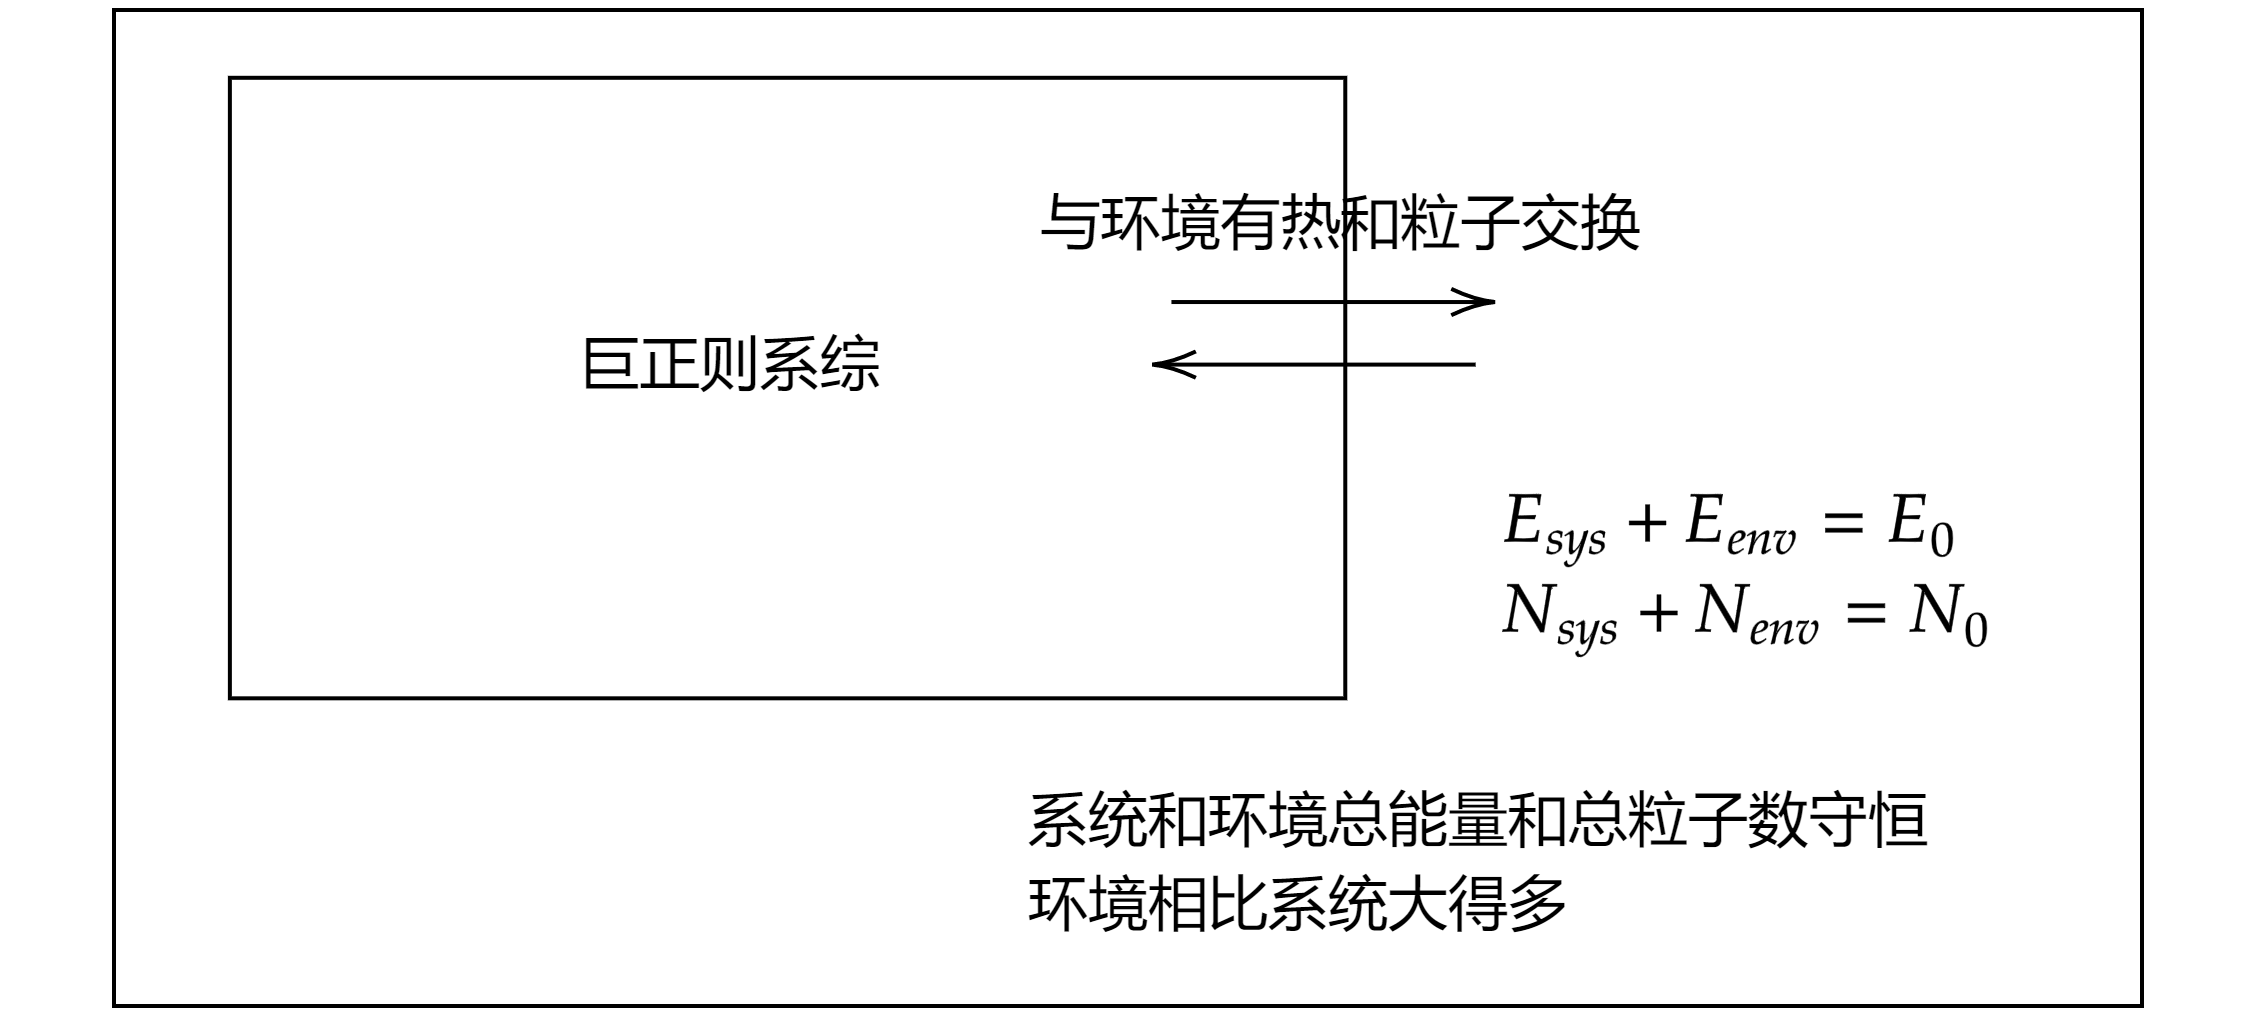
\includegraphics[width=0.6\textwidth]{fig/巨正则系综.png} 
      \caption{巨正则系综}
\end{figure}


和任一微观态的概率 $p_v$ 为\begin{equation}
       p_v=\frac{e^{-\beta E_v-\mu N_v}}{\Xi}
\end{equation}
其熵的表达式为\begin{equation}
       S=k_B (\ln \Xi+\beta E-\beta\mu N)=k_B \ln \Xi +\frac{E-\mu N}{T}
\end{equation}

从其熵的表达式我们不难得到\begin{equation}
       k_B T\ln \xi =TS -E+\mu N=-A+G =pV
\end{equation}
即$pV=k_BT \ln \Xi$,因此就有\begin{equation}
       \di (pV)=p\di V+V\di p=k_B T \di \ln \Xi+k_B\ln \xi \di T
\end{equation}
我们已知系统的$\mu,V,T$,利用$\ln \Xi$可以直接求出\begin{align}
       E&=\braket{E}=-\diffp*{\ln \Xi}{\beta}{\zeta, V}\\
       N&=\braket{N}=-\diffp*{\ln \Xi}{{(-\beta\mu)}}{\beta,V}\\
       S&=k_B \ln \Xi +\frac{E-\mu N}{T}\\
\end{align}
为了求出其他热力学量,我们利用\begin{equation}
       \di \ln \Xi =\beta p \di V+\beta V\di p -k_B \beta \ln \Xi \di T 
\end{equation}
而\begin{equation}
       \di G=\mu \di N+N\di \mu=V\di p -S\di T +\mu \di N
\end{equation}
所以$V\di p =S\di T +N\di \mu $,于是有\begin{equation}
       \di \ln \Xi =\beta p \di V+\beta (S-K_B \ln \Xi)\di T +\beta N \di \mu
\end{equation}
进而有\begin{equation}
       p=k_B T \diffp*{\ln \Xi}{V}{\mu,T}
\end{equation}

接下来我们讨论$E$和$N$的涨落,在正则系综中,我们有结论\begin{equation}
       \braket{(\Delta E)^2}=kT^2 \diffp{\braket{E}}{T}=kT^2 C_V
\end{equation}
对于$N$的涨落,我们有\begin{equation}
       \braket{(\Delta N)^2}=\diffp*{\braket{N}}{{(\beta\mu)}}{\beta,V}=kT \diffp*{\braket{N}}{\mu}{V,T}
\end{equation}

由数学结论\begin{equation}
       \diffp*{x}{y}{z} \diffp*{y}{z}{x}\diffp*{z}{x}{y}=-1
\end{equation}

所以就有\begin{equation}
       \diffp*{N}{\mu}{V,T}\cdot \diffp*{\mu}{V}{N,T}\cdot \diffp*{V}{N}{\mu,T}=-1
\end{equation}
所以\begin{equation}
       \diffp*{N}{\mu}{V,T}=-\diffp*{V}{\mu}{N,T}\cdot \diffp*{N}{V}{\mu,T}
\end{equation}
注意到\begin{equation}
       \di G=V\di p -S\di T +\mu \di N=\mu \di N+N\di \mu
\end{equation}
所以就有 \begin{equation}
       N\di \mu=V\di p-S\di T
\end{equation}
因此有Maxwell关系\begin{equation}
    \diffp{\mu}{p}=\diffp{V}{N}   
\end{equation}
以及\begin{equation}
       \diffp*{\mu}{p}{T}=\frac{V}{N}
\end{equation}
因此\begin{equation}
       \diffp*{V}{N}{T,\mu}=\frac{V}{N}
\end{equation}
所以\begin{equation}
       \diffp*{N}{\mu}{V,T}=-\frac{N}{V}\diffp*{V}{\mu}{N,T}=-\frac{N}{V} \left(\diffp{V}{p}\diffp{p}{\mu}\right)_{N,T}=-\frac{N^2}{V^2} \diffp*{p}{V}{N,T}=\frac{N^2}{V}\kappa
\end{equation}
其中\begin{equation}
       \kappa=\frac{1}{V}\diffp*{p}{V}{N,T}
\end{equation}
我们称为体变模量\index{体变模量}。所以\begin{equation}
       \braket{(\Delta N)^2}=kT \diffp*{\braket{N}}{\mu}{V,T}=\frac{kTN^2\kappa}{V}
\end{equation}
% subsection 巨正则系综的热力学关系 (end)
\subsubsection{$N$的巨正则分布} % (fold)
\label{ssub:N的巨正则分布}
因为任意微观态的概率为
\begin{equation}
       p_v=\frac{1}{\displaystyle \Xi} \exp\left(-\frac{E_v-\mu N_v}{kT}\right)
\end{equation}
并且\begin{equation}
       N_v=N_v(E_v,V)
\end{equation}
所以\begin{equation}
       p(N_v=N)=\sum_{v,\,N_v=N} p_v=\frac{e^{\beta\mu N}}{\displaystyle \Xi} \sum_{v,\,N_v=N} e^{-\beta E_v(N,v)} =\frac{e^{\beta\mu N}}{\displaystyle \Xi} Q(N,V,T)
\end{equation}
因此\begin{equation}
       \ln p(N) =\beta\mu N -\ln \Xi(\mu,V,T) +\ln Q(N,V,T)
\end{equation}
对$\ln p(N)$在$\braket{N}$附近做Taylor展开,可以得到\begin{equation}
       \ln p(N) =\ln p(\braket{N})+\left.\diffp{\ln p(\braket{N})}{N}\right|_{\braket{N}}(N-\braket{N}) +\left.\frac{1}{2}\diffp[2]{\ln p(\braket{N})}{N}\right|_{\braket{N}} (N-\braket{N})^2 +o(N^2)
\end{equation}

考虑到\begin{equation}
       \diffp{\ln p(N)}{N}=\beta \mu +\diffp*{\ln Q}{N}{V,T}=\beta\mu-\beta\mu=0
\end{equation}
而\begin{equation}
       \diffp[2]{\ln p(N)}{N}=\diffp*{\ln Q}{{N^2}}{V,T}
\end{equation}
因此\begin{equation}
       \left.\frac{1}{2}\diffp[2]{\ln p(\braket{N})}{N}\right|_{\braket{N}}=\diffp{{-\beta \mu }}{{\langle N\rangle} }=-\frac{1}{\braket{(\Delta N)^2}}
\end{equation}
也即\begin{equation}
       \ln p(N)= \ln p(\braket{N})-\frac{1}{2}\frac{(N-\braket{N})}{\braket{(\Delta N)^2}}
\end{equation}
因此$N$的概率分布为\begin{equation}
      p(N)=p(\braket{N})\exp\left(-\frac{(N-\braket{N})^2}{2\sigma_N^2}\right)
\end{equation}
% subsubsection $N$的巨正则分布 (end)
\subsubsection{热力学极限情形} % (fold)
\label{ssub:热力学极限情形}
考虑$N=\braket{N}$的时候\begin{equation}
       \Xi (\mu,V,T)=\sum_{v,\,N_v=\braket{N}} e^{-\beta E_v}=\sum_{v,\,N_v=\braket{N}} e^{-\beta E_v(\braket{N},v)}=e^{\beta\mu \braket{N}}Q(\braket{N},V,T)
\end{equation}
这个时候\begin{equation}
       k_BT \ln \Xi =pV =\mu N +k_BT \ln Q(\braket{N},V,T)=G-A
\end{equation}
是自洽的。
% subsubsection 热力学极限情形 (end)
% subsection 巨正则系综 (end)
\subsection{等温等压系综} % (fold)
\label{sub:等温等压系综}
等温等压系综的状态参量为$N,p,T$,有配分函数\begin{equation}
       \mathcal{Z}=(\beta p,N,\beta) =\sum_{v} e^{-\beta E_v-\beta pV_v}
\end{equation}
以及相对应的熵\begin{equation}
       S=k_B\ln \mathcal{Z} +\frac{E+pV}{T}
\end{equation}
核心热力学关系\begin{equation}
       k_BT\ln \mathcal{Z}=TS-E-pV=TS-H
\end{equation}
即\begin{equation}
       G=-k_B T\ln \mathcal{Z}
\end{equation}
其他的推导都是类似的,在这里就不赘述了

\begin{review}
       \item 正则系综的定义、状态参量;
       \item 配分函数的定义及其应用;
       \item 能量的涨落、正则分布;
       \item Sackur‐Tetrode 方程;
       \item Gibbs熵的定义;
       \item Gibbs熵和与Boltzman熵的联系;
       \item 广义系综的定义;
       \item 广义配分函数;
       \item 巨正则系综的定义;
       \item 粒子数的巨正则分布;
\end{review}
% subsection 等温等压系综 (end)
% section 广义系综 (end)
\section{习题} % (fold)
\label{sec:习题2}
\begin{enumerate}
       \item We know that the free energy  $F(T, V, N)$  of a thermodynamic system is extensive. Show that

       \[N\left(\frac{\partial F}{\partial N}\right)_{T, V}+V\left(\frac{\partial F}{\partial V}\right)_{T, N}=N f=F\]
       
       with  $f$  the free energy density expressed in suitable variables. Given this result, from the differential properties of  $F(T, V, N)$ , show that
       
       \[\Phi=N \mu\]
       
       with  $\Phi$  the Gibbs potential defined as $\Phi=F+P V $. In the above expression, $ \mu $ is the chemical potential properly defined in terms of $ F(T, V, N) $.
\end{enumerate}
% section 习题 (end)
% chapter 正则系综和广义系综 (end)
%---------------------------------------------------------------------------
% ----
\chapter{量子统计学的表述形式} 
\label{cha:量子统计学的表述形式}
\section{Introduction} % (fold)
\label{sec:quantIntroduction}
前面我们所讨论的系综理论是具有一般性的,当我们将其应用于经典系统的时候,不会有任何问题。但是当我们将它应用于由不可分辨的实体组成的量子系统的时候,就必须非常小心。

在这种情况下, 比较合适的方法是使用更加适合于量子力学的算符和波函数语言来改写系综理论。



% section Introduction (end)

\section{密度矩阵} % (fold)
\label{sec:密度矩阵}
如果系综中总共有$\mathcal{N}$个系统,第$k$个系统的波函数为$\psi^k(\bd{r},t)$,存在一个正交函数的完全集合$\varphi_n(\bd{r})$,使得我们可以将$\psi(\bd{r},t)$写成\begin{equation}
    \psi^k(\bd{r},t)=\sum_i a^k_n(t)\, \varphi_n(\bd{r})
\end{equation}
考虑一个物理量的系综平均,就有\begin{equation}
    \braket{A}_t=\frac{1}{\mathcal{N}}\sum_{k=1}^{N} \braket{\psi^k(t)|A|\psi^k(t)}=\frac{1}{\mathcal{N}}\sum_{k=1}^{N} \braket{\psi^k(t)|A|\psi^k(t)}.
\end{equation}

波函数随着时间的演化满足薛定谔方程\begin{equation}
    \hat{H}\psi^k(\bd{r},t)=i\hbar \dot{\psi}^k(\bd{r},t)
\end{equation}


于是我们定义密度算符\index{密度算符} $\hat{\rho}$
\begin{equation}
    \hat{\rho}(t)=\sum_{k}p_k \ket{\psi^k(t)}\bra{\psi^k(t)}
\end{equation}
其矩阵元为\begin{equation}
    \rho_{mn}(t)=\frac{1}{\mathcal{N}} \sum_{k=1}^{\mathcal{N}} a_{m}^k(t)a_n^k (t).
\end{equation}

一般来说,密度算符具有以下的性质
\begin{pointlist}{密度矩阵的性质}
    \begin{itemize}
        \item 密度矩阵的对角元由下式给出\begin{equation}
            \rho_{\alpha\alpha} =\sum_k p_k\ket{\alpha} \bra{\varphi^{k}(t)}\ket{\varphi^k(t)}\bra{\alpha} =\sum_k p_k \braket{\alpha|\varphi^k(t)}^2\le 1
        \end{equation}
        \item 密度矩阵的迹和时间无关,而且始终是归一化的\begin{equation}
            \operatorname{Tr} (\rho) = \sum_{\alpha} \rho_{\alpha\alpha}=1
        \end{equation}
        \item 密度矩阵的平方的迹总是小于1\begin{equation}
            \operatorname{Tr} (\rho^2) \le 1
        \end{equation}
        等号在系综由纯态组成的时候成立。
    \end{itemize}
\end{pointlist}

\begin{definition}
    从密度矩阵出发,可以定义von Neumann 熵\index{von Neumann 熵} \begin{equation}
        S=-\operatorname{Tr} \hat{\rho} \ln \hat{\rho} =-\sum_{\alpha} \lambda_\alpha \ln \lambda_{\alpha}
    \end{equation}
    其中$\lambda_\alpha$是密度矩阵的特征值。
\end{definition}


在系综理论中一个物理量的期望值应该由双重平均过程给出\begin{equation}
    \braket{G}=\frac{1}{\mathcal{N}}\sum_{k=1}^{\mathcal{N}} \braket{\psi^k(t)|G|\psi^k(t)}
\end{equation}
从而我们就有\begin{equation}
    \braket{G}=\frac{1}{\mathcal{N}} \sum_{k=1}^{\mathcal{N}} \left[\sum_{m,n} a_n^{k*}a_m^k G_{nm}\right]
\end{equation}
其中\begin{equation}
    G_{nm}=\int \varphi_n^* \hat{G} \varphi_m \di \tau
\end{equation}
于是任意一个物理量的平均值就可以写成\begin{equation}
    \braket{G}=\sum_{m,n} \rho_{mn}G_{nm}=\mathrm{Tr} (\hat{\rho}\hat{G}) 
\end{equation} 

考虑密度矩阵对时间的微分\begin{equation}
    \diffp{\rho}{t}= \sum_{k}p_k \left(\ket{{\diffp{{\psi^k}}{t}}}\bra{{\psi^k}}+\ket{{\psi^k}}\bra{\diffp{{\psi^k}}{t}}\right)
\end{equation}
利用薛定谔方程,我们就有\begin{equation}
    ih\diffp{\rho}{t}= \sum_{k}p_k \left(\hat{H}\ket{{\psi^k}}\bra{{\psi^k}}-\ket{{\psi^k}}\bra{{\psi^k}}\hat{H}\right)
\end{equation}
所以密度矩阵$\rho$满足\begin{equation}
    \dot{\rho} =-\frac{i}{\hbar} \left[\hat{H},\hat{\rho}\right]
\end{equation}
这就是经典的刘维尔方程的量子比拟。 
% section 密度矩阵 (end)
\section{各种统计系综} % (fold)
\label{sec:各种统计系综}
\subsection{微正则系综} % (fold)
\label{sub:quantum 微正则系综}
微正则系综的状态参量是$N,V,E$,即粒子数为$N$,体积为$V$,能量在$\displaystyle \left(E-\frac12\Delta, E+\frac12\Delta\right)$,其中$\Delta \ll E$。系统有$\Omega(N,V,E,\Delta)$每一个可及的态的概率相同。于是自然有密度矩阵\begin{equation}
    \rho = \frac{1}{\Omega(N,V,E,\Delta)} \sum_{k=1}^{\Omega(N,V,E,\Delta)} \ket{\psi^k(t)}\bra{\psi^k(t)}
\end{equation}

特别地$\Omega=1$的时候,我们称之为纯态
% subsection 微正则系综 (end)
\subsection{正则系综} % (fold)
\label{sub:quantum 正则系综}
在正则系综中,体系处于某一个状态的概率和$\exp(-\beta E_r)$成正比,于是可以归一化得到\begin{equation}
    \rho_n = \frac{\exp(-\beta E_n)}{\mathcal{Z}},\quad \mathcal{Z}=\sum_{n=1}^{\infty} \exp(-\beta E_n)
\end{equation}
进而正则系综的密度函数可以被写成\begin{equation}
    \begin{aligned}
        \rho(E) &= \sum_{n} \frac{\exp(-\beta E_n)}{\mathcal{Z}}   \ket{\varphi_n}\bra{\varphi_n}\\
        &= \sum_{n}\frac{\exp(-\beta E_n)}{\mathcal{Z}}   \ket{\varphi_n}\bra{\varphi_n}\\
        & =\frac{\exp(-\beta \hat{H})}{\operatorname{Tr}( \exp(-\beta \hat{H}))}
    \end{aligned}
\end{equation}
其中$\displaystyle \sum_n \bra{\varphi_n}\ket{\varphi_n}$为单位算符,而算符$\exp(-\beta \hat{H})$表示的是级数展开的结果\begin{equation}
    \exp(-\beta \hat{H})=\sum_{n=0}^{\infty} \frac{(-\beta \hat{H})^n}{n!}
\end{equation}

物理量的均值可以由下式给出\begin{equation}
    \braket{G}_N=\operatorname{Tr} (\hat{\rho}\hat{G}) =\frac{\operatorname{Tr}(\hat{G} \exp(-\beta \hat{H}))}{\operatorname{Tr}(\exp(-\beta \hat{H}))}
\end{equation}
% subsection 正则系综 (end)
\subsection{巨正则系综} % (fold)
\label{sub:quantum 巨正则系综}
巨正则系综相比正则系综释放了粒子数的限制,我们直接类比正则系综中的结论来得到巨正则系综的密度算符\begin{equation}
    \hat{\rho}=\frac{\exp[-\beta( \hat{H}-\mu\hat{n})]}{\mathcal{Q}(\mu,V,T)}=\frac{\exp(-\beta( \hat{H}-\mu\hat{n}))}{\operatorname{Tr}\{\exp[-\beta (\hat{H}-\mu \hat{n})]\}}
\end{equation}
% subsection 巨正则系综 (end)

% section 各种统计系综 (end)
\section{Examples} % (fold)
\label{sec:Examples}
我们来具体的看几个使用量子统计方法处理的例子。

\subsubsection{1.磁场中的一个电子}
\subsubsection{2.三维势箱中的一个自由粒子}
% section Examples (end)
\begin{review}
    \item 密度矩阵和密度矩阵的演化方程;
    \item von Neumann 熵;
    \item 系综的量子力学描述;
    \item 量子统计的实例;
\end{review}
\section{习题} % (fold)
\label{sec:习题3}
\begin{enumerate}
    \item 
\end{enumerate}
% section 习题 (end)
% chapter 量子统计学的表述形式 (end)
%---------------------------------------------------------------------------
%---------------------------------------------------------------------------
\chapter{Particles I (Theory)} % (fold)
\label{cha:particles I (Theory)}
\section{Introduction} % (fold)
\label{sec:introduction}
接下来我们将从抽象的系综理论过渡到具体的粒子构成的系统。相当于讨论系综理论的应用。

在开始讨论之前值得稍微区分的概念是关联\index{关联}(correlation)和相互作用\index{相互作用}(interacton)。相互作用一般会涉及到力和能量,可以被写进哈密顿量,关联指的是相互之间的一种关系,是比相互作用更大的概念,比如由于泡利不相容原理带来的两个电子不能具有完全相同的量子数,不能被写进哈密顿量。

\subsection{无关联系统} % (fold)
\label{sub:无关联系统}
我们先来讨论一下粒子之间无关联的情形,无关联,也就意味着粒子与粒子之间没有任何约束关系。显然稀薄的理想气体分子之间没有相互作用,因此是一个无关联系统。接下来我们以理想气体分子为例,讨论一下无关联系统。

我们将体积$V$分成m个格子,由于气体充分地稀薄,我们可以认为每个格子中至多有一个粒子,每个格子上粒子的占据数记为$n_i$,因此\begin{equation}
    n_i=0,1.
\end{equation}
因此每一组$\{n_i\}$就对应于一个微观态。
粒子总数$N$满足\begin{equation}
    N=\sum_i^m n_i.
\end{equation}
因此就有\begin{equation}
    \braket{N}=\sum_i^m \braket{n_i}.
\end{equation}
而\begin{equation}
    \braket{(\Delta N)^2} =\braket{N^2}-\braket{N}^2
\end{equation}
注意到\begin{equation}
    N^2=\sum_i^m \sum_j^m n_i n_j.
\end{equation}
所以 \begin{equation}
    \braket{N^2}= \sum_i^m \sum_j^m \braket{n_i n_j}.
\end{equation}
考虑理想气体分子之间的无关联性,因此\begin{equation}
    \braket{n_i n_j}= \braket{n_i}\braket{n_j} \quad \text{for}\ i\neq j.
\end{equation}
进而我们就有\begin{equation}
    \begin{aligned}
        \braket{(\Delta N)^2} & =\sum_i^m \sum_j^m \braket{n_i n_j}-\sum_i^m \sum_j^m \braket{n_i}\braket{n_j} \\
                              & =\sum_i^m  \braket{n_i^2}-\sum_i^m \braket{n_i}^2                              \\
    \end{aligned}
\end{equation}
注意到$n_i^2=n_i=1$,因此就有 \begin{equation}
    \begin{aligned}
        \braket{(\Delta N)^2} & =\sum_i^m  \braket{n_i}-\sum_i^m \braket{n_i}^2 \\
                              & =\sum_i^m  \braket{n_i}(1- \braket{n_i})        \\
    \end{aligned}
\end{equation}
考虑到气体比较稀薄,因此\begin{equation}
    \braket{n_i}\ll 1.
\end{equation}
从而\begin{equation}
    \braket{(\Delta N)^2}= \sum_i^m  \braket{n_i}(1- \braket{n_i})    \approx \sum_i^m  \braket{n_i}=\braket{N}.
\end{equation}
于是对于无关联理想气体就有\begin{equation}
    \braket{N}=\braket{(\Delta N)^2} =\diffp*{{\braket{N}}}{{(\beta \mu)}}{\beta,V}
\end{equation}
在巨正则系综中,$T$和$V$固定,理想气体的密度可以表示为\begin{equation}
    \rho=\frac{\braket{N}}{V}.
\end{equation}
因此\begin{equation}
    \diffp*{{\rho}}{{(\beta \mu)}}{\beta,V} =\rho
\end{equation}
由热力学结论\begin{equation}
    \di \mu =\frac{V}{N} \di p=\frac{\di \rho}{\rho}
\end{equation}
因此\begin{equation}
    \rho=\diffp{p}{\mu}=\diffp{\rho}{{\beta \mu}}
\end{equation}
因此\begin{equation}
    \beta \diffp{p}{\rho}=1
\end{equation}
积分可以得到\begin{equation}
    \frac{p}{k_B T}=\rho+C
\end{equation}
容易验证$C=0$,于是我们就得到了理想气体状态方程\begin{equation}
    pV=Nk_BT
\end{equation}
于是立足于无关联假设和一点巨正则系综的结论,我们就可以导出理想气体状态方程。
特别地,利用
\begin{equation}
    \diffp*{{\rho}}{{(\beta \mu)}}{\beta,V} =\rho
\end{equation}
可以直接积分得到化学势的表达式\index{化学势}\begin{equation}
    \beta \mu =\ln \rho +C(T,V)
\end{equation}
因此\begin{equation}
    \mu=kT\ln p +C_1(T,V)
\end{equation}
设\begin{equation}
    \mu^{\ominus} =kT\ln p^{\ominus} +C_1(T,V)
\end{equation}
于是\begin{equation}
    \mu =\mu^\ominus +kT \ln \frac{p}{p^\ominus}
\end{equation}
% subsection 无关联系统 (end)
\subsection{配分函数因子化} % (fold)
\label{sub:配分函数因子化}
我们以最简单的正则配分函数为例\begin{equation}
    Q=\sum_v e^{-\beta \mu_v}
\end{equation}
假设每个微观态的能量都可以被分为若干不可区分且独立无关联的部分\begin{equation}
    E_v =\sum_i E_{vi}
\end{equation}
这个时候每一个微观态其实就对应于一组$\{vi\}$,因此\begin{equation}
    Q=\sum_{\{vi\}} \exp{(-\beta \sum_i E_{vi})}=\prod_i \sum_{v_i} \exp{(-\beta E_{vi})}
\end{equation}
也可以写作\begin{equation}
    Q=\prod_i Q_i
\end{equation}
其中$\displaystyle Q_i=\sum_{vi}e^{-\beta E_{vi}}$。
某一个微观态出现的概率也可以按照\begin{equation}
    p_v=\frac{e^{-\beta \mu_v}}{Q}= \frac{\prod_i e^{-\beta E_{vi}}}{\prod_i Q_i}=\prod_i p_{vi}
\end{equation}
我们刚才求积的过程就是配分函数因子化\index{配分函数因子化}。从配分函数的因子化出发,我们可以分解系综平均和涨落。

基于这些结论我们就可以来分析一个实际的$N$粒子系统。

% subsection 配分函数因子化 (end)
\subsection{全同粒子} % (fold)
\label{sub:全同粒子}
$N$个粒子的能级可以直接拆分开来\begin{equation}
    E_v=\sum_{i=1}^N E_{vi}
\end{equation}
于是\begin{equation}
    Q=Q_1^N
\end{equation}
其中单粒子的配分函数为\begin{equation}
    Q_1=\sum_{v_1} e^{-\beta E_{v_1}}=\sum_j g_j e^{-\beta E_j}
\end{equation}
但是考虑到粒子的全同性,以及稀薄假设:态的数目远远大于粒子数,两个粒子不会基本占据同一个态。因此就有\begin{equation}
    Q=\frac{Q_1^N}{N!}
\end{equation}
% subsection 全同粒子 (end)
% section introduction (end)
\section{量子统计理论} % (fold)
\label{sec:量子统计理论}
\subsection{Bose-Einstein统计和Fermi-Dirac统计} % (fold)
\label{sub:Bose-Einstein统计和Fermi-Dirac统计}
从量子力学的角度出发,全同性原理可以被表述成,交换任意两个全同粒子,其波函数在空间中的概率密度分布不会改变,也就是\begin{equation}
    |\hat{P}_{12}\psi(1,2)|^2=|\psi(1,2)|^2=|\psi(2,1)|^2
\end{equation}
因此$\hat{P}_{12}$的本征值应该是$\pm 1$。当$\psi(1,2)=\psi(2,1)$的时候,我们称之为玻色子,当$\psi(1,2)=-\psi(2,1)$的时候,我们称之为费米子。费米子满足Pauli不相容原理\index{Pauli不相容原理}:两个全同的费米子不能处于完全相同的量子态,于是对于玻色子,其某一个能级的占据数$n_k$可能是$0,1,2,...$,而对于费米子,只能是$1$或者$2$。

假设不存在简并能级玻色子和费米子在0K时的能级分布如图\ref{fig:boson and fermion}所示。这个时候对于费米子而言,最高已占据的能级就是费米能级\index{费米能级}。其定义如下\begin{definition}
    假设把所有的费米子从这些量子态上移开。之后再把这些费米子按照泡利不相容原理填充在各个可供占据的量子态上,并且这种填充过程中每个费米子都占据最低的可供占据的量子态。最后一个费米子占据着的量子态 就是费米能级。
\end{definition}
\begin{figure}[h]
    \centering
    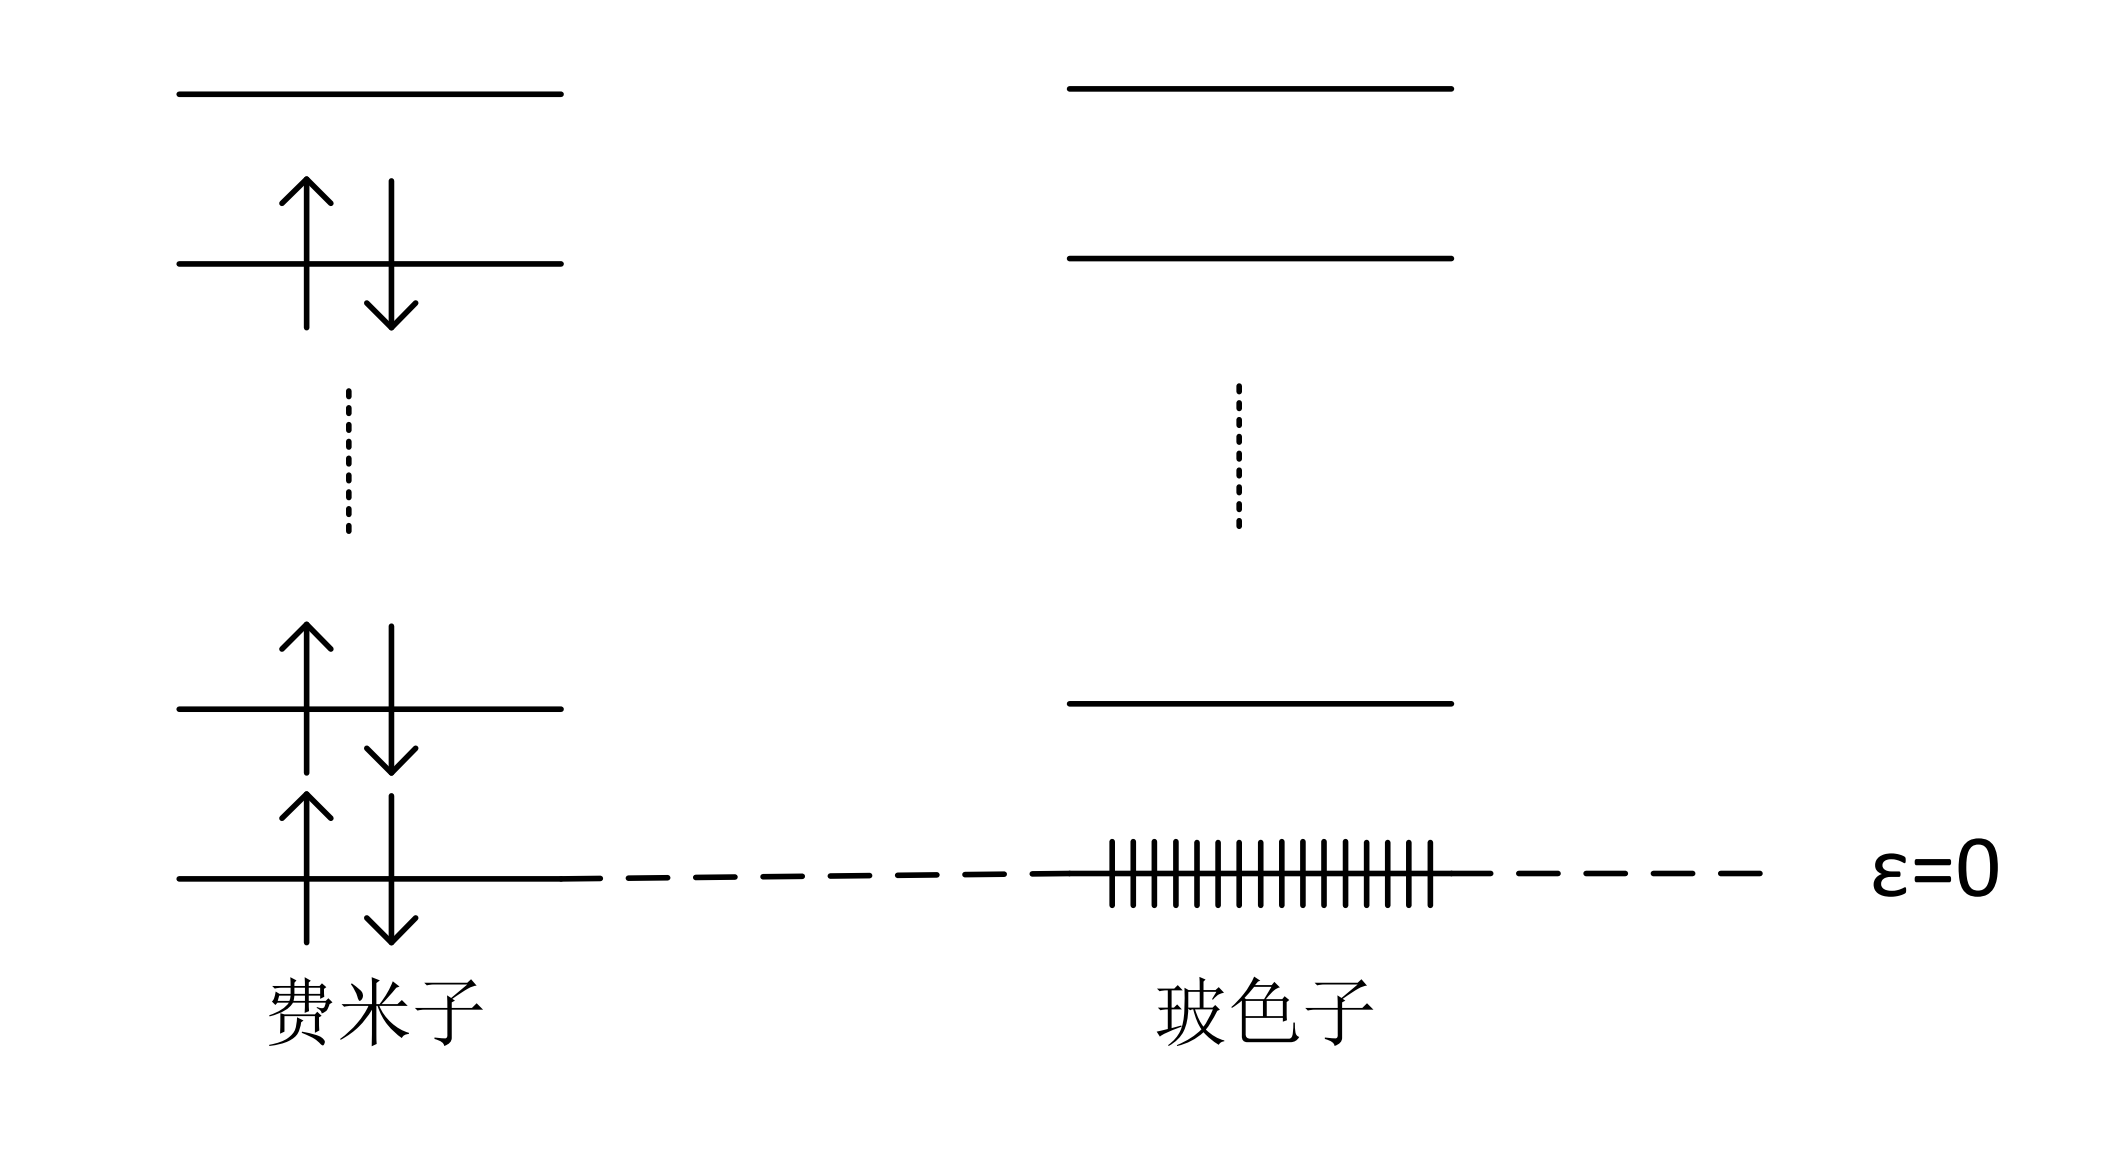
\includegraphics[width=0.64\textwidth]{fig/boson and fermion.png}
    \caption{玻色子和费米子的能级分布}
    \label{fig:boson and fermion}
\end{figure}
事实上,费米子的性质也主要由Fermi能级附近的粒子决定。

当$T>0K$的时候,粒子受热激发会跃迁到更高的未占据能级上。对于费米子,只有Fermi能级附近的粒子会受到激发,因此熵增只在很小的尺度上,而玻色子则会有宏观量级的粒子受到激发,随着温度的上升,玻色子的熵会快速增加。考虑化学势\begin{equation}
    \mu =\diffp*{E}{N}{S,V}
\end{equation}
低温情形下,对费米子新的粒子加入到费米能级附近,熵和体积都几乎不变,因此\begin{equation}
    \mu \sim E_F
\end{equation}
而对于玻色子新的粒子加入进来,就会有熵增,如果要维持熵不变,那么就需要降低体系的温度,因此保持$S$不变$N$增大,体系的能量会变小,于是\begin{equation}
    \mu = \diffp*{E}{N}{S,V}< 0
\end{equation}
在高温情形下,费米子和玻色子的熵都会随着体系的粒子数增加而增加,因此\begin{equation}
    \mu = \diffp*{E}{N}{S,V}< 0
\end{equation}

现在我们再回到统计力学的研究框架下,我们使用巨正则系综,令体系的$k$能级上的粒子占据数为$n_k$,于是粒子数\begin{equation}
    N_v=\sum_{k} n_k
\end{equation}
所以配分函数满足\begin{equation}
    \Xi =\sum_v e^{-\beta (E_v -\mu N_v)}=\sum_{\{n_k\}} e^{-\beta \sum_k n_k E_k +\beta \mu \sum_k n_k}=\sum_{\{n_k\}}\left[ \prod_k \left(e^{-\beta(\varepsilon_k-\nu)}\right)^{n_k}\right]
\end{equation}
求和和连乘可以交换,于是\begin{equation}
    \Xi =\prod_{k} \left[\sum_{n_k} \left(e^{-\beta(\varepsilon_k-\mu)}\right)^{n_k}\right] =\prod_k \Xi_k
\end{equation}
于是一个微观态的概率为\begin{equation}
    p_v =p_{\{n_k\}}=\frac{e^{-\beta (E_v -\mu N_v)}}{\Xi}=\frac{\prod_k e^{-\beta(\varepsilon_k-\mu)n_K}}{\prod_k\Xi_k}=\prod_k p_{n_k}
\end{equation}
于是原本\textbf{求体系的巨配分函数的工作就变成了求某一个状态的配分函数}。这就要简单了很多。对于费米子,$n_k$只能取$0$或者$1$,因此\begin{equation}
    \Xi_k=1+e^{-\beta(\varepsilon_k-\mu)}
\end{equation}
对于玻色子,$n_k$可以取$0,1,2,...$,因此\begin{equation}
    \Xi_k=\sum_{n_k=0}^{\infty} e^{-\beta(\varepsilon_k-\mu)n_k}=\frac{1}{1-e^{-\beta(\varepsilon_k-\mu)}}
\end{equation}
于是巨配分函数可以表示为\begin{equation}
    \Xi =\prod_k \Xi_k=\prod_k \left[1-e^{-\beta(\varepsilon_k-\mu)}\right]^{\pm 1}
\end{equation}

在此基础上,我们可以考量一个态的\textbf{平均占据数}\index{平均占据数},即\begin{equation}
    \langle n_k\rangle =\sum_{n_k} n_k p_{n_k}=\sum_{n_k} n_k \frac{e^{-\beta n_k (\varepsilon_k-\mu)}}{\Xi_{k}}=-\frac1\beta \frac{\partial \ln \Xi_k}{\partial \varepsilon_k}
\end{equation}
对于费米子这个结果为\begin{equation}
    \langle n_k\rangle =\frac{1}{e^{\beta(\varepsilon_k-\mu)}+1}
\end{equation}
对于玻色子,结果为\begin{equation}
    \langle n_k\rangle =\frac{1}{e^{\beta(\varepsilon_k-\mu)}-1}
\end{equation}

我们已经分析了占据数的系综平均,接下来我们稍微看一下占据数的涨落$\braket{(\Delta n_k)^2}$。首先我们考虑$\braket{\Delta n_k \Delta n_k'}$\begin{equation}
    \begin{aligned}
        \braket{\Delta n_k \Delta n_{k'}} & =\braket{(n_k-\braket{n_k})(n_{k'}-\braket{n_{k'}})} \\
        & =\braket{n_k n_{k'}}-\braket{n_k}\braket{n_{k'}}  \\
        & = \frac{1}{\beta^2}\left( \frac{1}{\Xi}\diffp{\Xi}{{\varepsilon_k }{\varepsilon_{k'}}} -\frac{1}{\Xi^2} \diffp{\Xi}{{\varepsilon_k}}\diffp{\Xi}{{\varepsilon_{k'}}}\right)\\
        & = \frac{1}{\beta^2}\diffp{}{{\varepsilon_k}}\left(\frac{1}{\Xi} \diffp{\Xi}{{\varepsilon_{k'}}}\right)\\
        & = \frac{1}{\beta^2}\diffp{\ln \Xi}{{\varepsilon_k }{\varepsilon_{k'}}}\\
        & = -\frac{1}{\beta}\diffp{{\braket{n_k}}}{{\varepsilon_{k'}}}
        =\begin{cases}
            0 & k\neq k' \\
            \braket{(\Delta n_k)^2} & k=k'
        \end{cases}
    \end{aligned}
\end{equation}
于是占据数的涨落为\begin{equation}
\begin{aligned}
    \braket{(\Delta n_k)^2}& =-\frac{1}{\beta}\diffp{{\braket{n_k}}}{{\varepsilon_{k}}} =-\frac{1}{\beta}\diffp{{(e^{\beta (\varepsilon_k-\mu)}\pm 1)^{-1}}}{{\varepsilon_{k}}} 
    & = \frac{e^{\beta (\varepsilon_k-\mu)}}{( e^{\beta (\varepsilon_k-\mu)}\pm 1)^{2}}=\braket{n_k}\mp \braket{n_k}^2
\end{aligned}\end{equation}

事实上对于费米子而言这个结果是比较显然的,因为$n_k=0,1$,所以$n_k^2=n_k$\begin{equation}
    \braket{n_k^2}-\braket{n_k}^2=\braket{n_k}-\braket{n_k}^2
\end{equation}

现在我们对我们前面得到的结论稍微做一点分析,比如平均占据数\begin{equation}
    \langle n_k\rangle =\frac{1}{e^{\beta(\varepsilon_k-\mu)}\pm 1}
\end{equation}
对于费米子,\begin{equation}
    \langle n_k\rangle =\frac{1}{e^{\beta(\varepsilon_k-\mu)}+1}
\end{equation}
显然$0\le \braket{n_k}\le 1$,当且仅当$T=0$K的时候,可以取到等号,此时\begin{equation}
    \braket{n_k}=\begin{cases}
        0 & \varepsilon_k>\mu \\
        1 & \varepsilon_k<\mu
    \end{cases}
\end{equation}
当$\varepsilon_k=\mu$的时候,$\braket{n_k}=\frac{1}{2}$,所以我们可以进一步的了解前面提到的费米能级:费米能级以下平均占据数都为1,以上占据数都为0,费米能级自己的平均占据数为$\frac{1}{2}$。

对于玻色子
\begin{equation}
    \braket{n_k}=\frac{1}{e^{\beta(\varepsilon_k-\mu)}-1}
\end{equation}
考虑到$\braket{n_k}$的物理意义,因此$\varepsilon_k\le \mu$恒成立。到这里,我们已经基本完成了对量子统计理论的讨论,接下来我们开始讨论经典统计的方法。
% subsection Bose-Einstein统计和Fermi-Dirac统计 (end)
\subsection{经典极限} % (fold)
\label{sub:经典极限}
经典统计最基本的认知就是前面讨论的:态的数目远远大于粒子的数目,完成了前面的讨论之后,我们有一种等价的说法$\braket{n_k}\ll 1$。

当$\braket{n_k}\ll 1$的时候,也就有$e^{\beta (\varepsilon_k-\mu)}\gg 1$,因此我们就有\begin{equation}
    \braket{n_k}=\frac{1}{e^{\beta(\varepsilon_k-\mu)}\pm 1}\approx e^{-\beta(\varepsilon_k-\mu)}
\end{equation}
这就是经典极限下的Maxwell-Boltzman分布。注意到此时\begin{equation}
    \braket{n_0} =e^{\beta \mu} \ll 1
\end{equation}
这也就是经典统计\index{经典统计}的一种等价说法,$e^{\beta \mu} \ll 1$,即$\mu$是一个绝对值很大的负数。

对于上述的Maxwell-Boltzman分布,我们有\begin{equation}
    \braket{N}=\sum_{k} \braket{n_k}=e^{\beta \mu} \sum_{k} e^{-\beta\varepsilon_k}=qe^{\beta \mu}
    \label{equ:N with exp beta mu}
\end{equation}
其中$q$为单粒子配分函数。因此\begin{equation}
    \frac{\braket{N}}{q}=e^{\beta \mu} \ll 1
\end{equation}
这就又是经典统计的等价表述:单粒子的配分函数远远大于粒子总数。其中,粒子处于状态$k$的概率为\begin{equation}
    p_k =\frac{\braket{n_k}}{\braket{N}}=\frac{e^{-\beta \varepsilon_k}}{q}
\end{equation}
这个结果和热力学中的结论是一致的。

% subsection 经典极限 (end)
\subsection{巨正则系综的应用} % (fold)
\label{sub:巨正则系综的应用}
介绍了两种统计方法之后,我们再回到巨正则系综的理论中来。考察一个多组分的体系,有\begin{equation}
\begin{aligned}
    \Xi &=\sum_v e^{\beta (\sum_i \mu_i N_i^v -E_v)}\\
    &=\sum_{\{N_i\}} e^{\beta \sum_i N_i} \sum_{N_i^v=N_i} e^{-\beta E_v} \\
    &=\sum_{\{N_i\}} e^{\beta \sum_i N_i} Q(T,V,N_i)
\end{aligned}
\end{equation}
取最概然近似,就有\begin{equation}
    \Xi \approx e^{\beta \sum_i \mu_i\braket{N_i}} Q(T,V,\braket{N_i})
\end{equation}
于是可以得到\begin{equation}
    \ln Q =\ln \Xi -\beta \sum_i \mu_i\braket{N_i}
    \label{equ:Q with Xi}
\end{equation}

另一方面,对一个粒子系统,有\begin{equation}
    N_i^v =\sum_{k_i} n_{k_i},\quad E^v=\sum_i\sum_{k_i}n_{k_i} \varepsilon_{k_i}
\end{equation}
代入巨正则系综配分函数的表达式可以得到\begin{equation}
   \begin{aligned}
    \Xi &=\sum_{\{n_{k_i}\}} e^{\sum_i\sum_{k_i}\beta(\mu_i-\varepsilon_{k_i})n_{k_i} } \\
    & = \prod_i \prod_{k_i} \left[\sum_{n_{k_i} }e^{\beta(\mu_i-\varepsilon_{k_i})n_{k_i} }\right]
    &= \prod_i \prod_{k_i} \left[1\pm e^{\beta(\mu_i-\varepsilon_{k_i})n_{k_i} }\right]
   \end{aligned}
\end{equation}
因为$e^{\beta (\mu_i -\varepsilon_{k_i})}\ll1$,利用当$x\to 0$的时候$\ln (1\pm x)\sim pm x$,于是\begin{equation}
    \ln \Xi \approx \sum_i \sum_{k_i} e^{\beta(\mu_i-\varepsilon_{k_i})}
\end{equation}
代入式\ref{equ:Q with Xi},我们就可以得到\begin{equation}
\begin{aligned}
    \ln Q &= \sum_i \sum_{k_i} e^{\beta(\mu_i-\varepsilon_{k_i})}- \beta \sum_i \mu_i\braket{N_i}
    &=\sum_i e^{\beta \mu_i} q_i - \beta \sum_i \mu_i\braket{N_i}\\
    &=\sum_i \left(e^{\beta \mu_i} q_i -\beta \mu_i\braket{N_i}\right)
    \label{equ:Q with exp beta mu qi and N}
\end{aligned}
\end{equation}
由式\ref{equ:N with exp beta mu},我们知道\begin{equation}
    e^{\beta \mu_i}=\frac{\braket{N_i}}{q_i}\ \Rightarrow \  \beta \mu_i =\ln\braket{N_i} -\ln q_i
\end{equation}
代入\ref{equ:Q with exp beta mu qi and N},我们可以得到\begin{equation}
    \begin{aligned}
        \ln Q &=\sum_i \left(\braket{N_i} -\braket{N_i}\ln \braket{N_i} +\braket{N_i}\ln q_i\right)\\
        & \approx \sum_i \left(\ln q_i^{N_i}-\ln N_i!\right)\\
        &=\sum_i \ln \frac{q_i^{N_i}}{N_i!}
    \end{aligned}
\end{equation}
也即\begin{equation}
    Q =\prod_i \frac{q_i^{N_i}}{ \ln N_i!}
\end{equation}
% subsection 巨正则系综的应用 (end)

% section 量子统计理论 (end)
\begin{review}
    \item 无关联系统的统计理论
    \item 配分函数因子化;
    \item 全同粒子;
    \item Bose-Einstein统计;
    \item Fermi-Dirac统计;
    \item 量子统计的经典极限;
    \item 巨正则系综的应用
\end{review}
\section{习题} % (fold)
\label{sec:习题4}

% section 习题 (end)
% chapter particles I (Theory) (end)


%---------------------------------------------------------------------------
%---------------------------------------------------------------------------
\chapter{Particles II (Application)} % (fold)
\label{cha:particles II (Application)}
\section{Photon and Phonon} % (fold)
\label{sec:photon_and_phonon}
\subsection{黑体辐射} % (fold)
\label{sub:黑体辐射}
\begin{definition}[黑体\index{黑体}]
    黑体,指的是能够完全吸收任何波长的外来辐射而无任何反射的物体。
\end{definition}

理想的黑体当然是不存在的,实验上可以用一个开了小孔的金属空腔来近似黑体(这里的黑体指的是这个孔,不是金属空腔本身)。

对于特定体积的容器$V$是固定的,由于我们只考察平衡态的情形,因此该体系需要与环境达成热平衡,即$T$一定。但是由于器壁会不断地吸收和释放光子,因此$N$是无法确定的。

\begin{remark}
    由于不同的电磁波之间发生直接转化,只能通过物质的吸收和发生来间接转化。因此表征物质转化趋势的化学势$\mu$在这里是没有意义的。所以我们直接取$\mu=0$。
\end{remark}

在进一步讨论之前,我们可以稍微回顾一下光子最重要也是最基本的性质——波粒二象性。

\subsubsection{波动性描述}

\begin{table}[h]
    \centering
    \begin{tabular}{cccccc}
        周期$T$ & 频率$\nu$ & 角频率 $\omega =2\pi \nu$ & 波长$\lambda$ & 波数$\widetilde{\nu}=\frac{1}{\lambda}$ & 波矢 $k=2\pi \widetilde{\nu}$ \\
    \end{tabular}
\end{table}

以及最关键的公式\begin{equation}
    \lambda \nu =c
\end{equation}
空间中的一个平面波可以表示为\begin{equation}
    \varphi=A\left[e^{i(\bd{k} \cdot \bd{r}-\omega t)}+\text{C.C.}\right]
\end{equation}

\subsubsection{粒子性描述}

光子的能量和动量分别为 \begin{equation}
    E=h\nu=\hbar \widetilde{\nu}, \quad \bd{p}=h\bd{k}
\end{equation}
利用平面波色散关系\begin{equation}
    \omega=ck
\end{equation}
就可以得到能量-动量关系\begin{equation}
    E=pc
\end{equation}

在光子气模型中$N$没有办法确定,因此$\mu$是没有意义的,我们的分析只能立足于$V,T$。这个时候巨正则配分函数和正则配分函数等价\begin{equation}
    \Xi =Q
\end{equation}

对于一个微观态$v$,它可以用不同的状态以及占据数来描述\begin{equation}
    v\leftrightarrow \{\omega_i , \bd{k}_i, g_i, n_i\}
\end{equation}
其中$\omega_i$,$\bd{k}_i$,$g_i$,$n_i$分别是频率、波矢、振动模式、占据数,由于光子是玻色子,所以$n_i$可以取任意自然数。微观态$v$的能量可以表示为\begin{equation}
    E_v=\sum_i n_i \hbar\omega_i
\end{equation}

我们知道,对于玻色子其配分函数为\begin{equation}
    \ln \Xi =-\sum_i \ln (1-e^{-\beta \varepsilon_i}),\quad (\mu=0)
\end{equation}
以及某一个能级的占据数\begin{equation}
    \braket{n_i}=\frac{1}{e^{\beta\varepsilon_i}-1}
\end{equation}
将这个结果应用于光子气,就有\begin{equation}
    \braket{E} =-\diffp{\ln \Xi}{\beta} =\sum_i \braket{n_i} \varepsilon_i=\sum_i \frac{\varepsilon_i}{e^{\beta\varepsilon_i}-1}
\end{equation}
其中$\varepsilon_i =n_i\hbar\omega_i$
实际的频率应该近似为一个连续分布,于是求和可以化成积分\begin{equation}
    \braket{E} =\int_0^\infty \frac{\varepsilon}{e^{\beta\varepsilon}-1} \rho(\varepsilon)\di\varepsilon
\end{equation}

\begin{remark}
    如果我们想要知道黑体的某一个能量区间中的光子密度,只需要知道这个态对应的驻波的种类数。一维情形下驻波的条件为\begin{equation}
        a=n\cdot \frac{\lambda}{2}
    \end{equation}
    所以\begin{equation}
        k=\frac{2\pi}{\lambda} =\frac{n\pi}{a}
    \end{equation}
    这个结论可以拓展到三维,于是就有\begin{equation}
        \bd{k}=\frac{\pi}{a} (n_x \bd{i}+n_y\bd{j}+n_z\bd{k})
    \end{equation}
    或者\begin{equation}
        k^2 =\frac{\pi^2}{a^2} (n_x^2+n_y^2+n_z^2)
    \end{equation}
    注意到\begin{equation}
        k=\frac{\omega}{c} =\frac{\varepsilon}{\hbar c}
    \end{equation}
    于是\begin{equation}
        n_x^2+n_y^2+n_z^2 =\frac{\varepsilon^2 a}{\pi\hbar^2 c^2} 
    \end{equation}
    因此能量介于$0\sim \varepsilon$之间的态的数量就等于\begin{equation}
        2\times\frac{1}{8} \times \frac{4}{3} \pi \left(\frac{\varepsilon}{\hbar c\pi}\right)^3=\frac{V}{6\pi^2} \frac{\varepsilon^3}{\hbar^3 c^3}
    \end{equation}
    上式中的因子2来自于偏振自由度,于是\begin{equation}
        \rho(\varepsilon) =\di\left(\frac{V}{3\pi^2} \frac{\varepsilon^3}{\hbar^3 c^3} \right) =\frac{V}{\pi^2}\frac{\varepsilon^2}{\hbar^3c^3} \di\varepsilon
    \end{equation}
\end{remark}

据此我们就可以进一步计算平均能量\begin{equation}
    \braket{E} =\int_{0}^{+\infty}\frac{V}{\pi^2}\frac{\varepsilon^2}{\hbar^3c^3} \frac{\varepsilon}{e^{\beta\varepsilon}-1}\mathrm{d}\varepsilon
\end{equation}
因为$\varepsilon=\hbar \omega$,所以\begin{equation}
    \braket{E} =\int_{0}^{+\infty}\frac{V}{\pi^2 c^3 }\frac{\hbar\omega^3}{e^{\beta\hbar\omega}-1} \mathrm{d}\omega
\end{equation}
其中\begin{equation}
    p_{T,V} =\frac{V}{\pi^2c^3} \frac{\hbar\omega^3}{e^{\beta \hbar\omega}-1}
\end{equation}
被称为黑体辐射的普朗克公式\index{黑体辐射的普朗克公式}。在此基础上,我们可以进行一些更加细致的分析。

对于高温低频的情形,$\displaystyle \frac{\hbar \omega}{kT}\ll 1$,整理后有\begin{equation}
    p_{T,V}=kT \omega^2 \frac{V}{\pi^2 c^3}
\end{equation}
这个公式被称为Rayleigh-Jeans公式,\index{Rayleigh-Jeans公式},此时主要表现为波动性。

对于低温高频的情形,$\displaystyle \frac{\hbar \omega}{kT}\gg 1$,整理后有\begin{equation}
    p_{T,V}=\frac{V}{\pi^2 c^3}\hbar \omega^3 e^{-\frac{\hbar \omega}{kT}}
\end{equation}
被称为Wien公式\index{Wien公式},其图形如图\ref{fig:wien equation}。这个时候主要表现为粒子性。不难发现$\omega_{\max}\propto T$,即黑体辐射谱的峰值位置只和温度有关,我们称之为Wien位移定律\index{Wien位移定律}。
\begin{figure}[h]
       \centering
       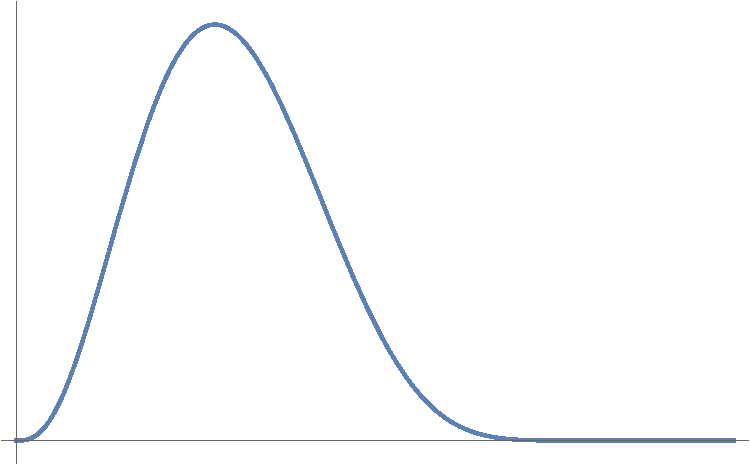
\includegraphics[width=0.6\textwidth]{fig/wien.pdf}
       \caption{黑体辐射的Wien公式}
       \label{fig:wien equation}
\end{figure}

重新考虑我们之前得到的$\braket{E}$,\begin{equation}
    \braket{E} =\frac{8\pi V}{h^2 c^3} \int_0^{+\infty} \frac{\varepsilon^3}{e^{\beta \varepsilon}-1}\di \varepsilon
\end{equation}
所以体积能量密度\begin{equation}
    \frac{\braket{E}}{V} = \frac{8\pi}{h^3 c^3 \beta^4} \int_0^{+\infty} \frac{x^3}{e^x -1} \di x=\frac{8\pi^5}{15h^3 c^3} (kT)^4
\end{equation}

考虑这个体系的配分函数,就有\begin{equation}
\begin{aligned}
    \ln \Xi &=-\sum_i \ln\left(1-e^{-\beta\varepsilon_i}\right)\\
    &= -\int_{0}^{+\infty}\ln (1-e^{-\beta \varepsilon} ) \rho(\varepsilon) \mathrm{d}\varepsilon\\
    & = -\int_{0}^{+\infty} \ln (1-e^{-\beta \varepsilon} )  \frac{8\pi v}{h^3 c^3}\varepsilon^2\mathrm{d}\varepsilon\\
    & = -\frac{8\pi V}{\beta^3 h^3 c^3} \int_{0}^{+\infty}\ln(1-e^{-x})x^2  \mathrm{d}x=-\frac{1}{3} \frac{8\pi^5 v \beta^{-3}}{45 h^3 c63}
\end{aligned}
\end{equation}

在配分函数的基础上,我们可以回顾一下之前的物理量:\begin{gather}
    \braket{E} = -\diffp{{\ln \Xi}}{{\beta}} =\frac{8\pi^5 V}{15h^3 c^3}(kT)^4\\
    p=\frac{kT}{V} \ln \Xi =\frac{8\pi^5}{45h^3 c^3}\beta^{-4}
\end{gather}
特别地,这里有\begin{equation}
    pV =\frac{1}{3}\braket{E}
\end{equation}

考虑到$\mu=0$,因此熵满足\begin{equation}
    S=k\ln \Xi +\frac{\braket{E}}{T} =4k\ln\Xi
\end{equation}
以及\begin{equation}
    A=E-TS =-kT \ln \Xi
\end{equation}
% subsection 黑体辐射 (end)
\subsection{声子} % (fold)
\label{sub:声子}
在金属晶体中,我们认为金属正离子在晶格位置附近振动,而电子弥散在电子海中。实验中我们观察到晶体的热容满足如下的规律:
\begin{figure}[h]
       \centering
       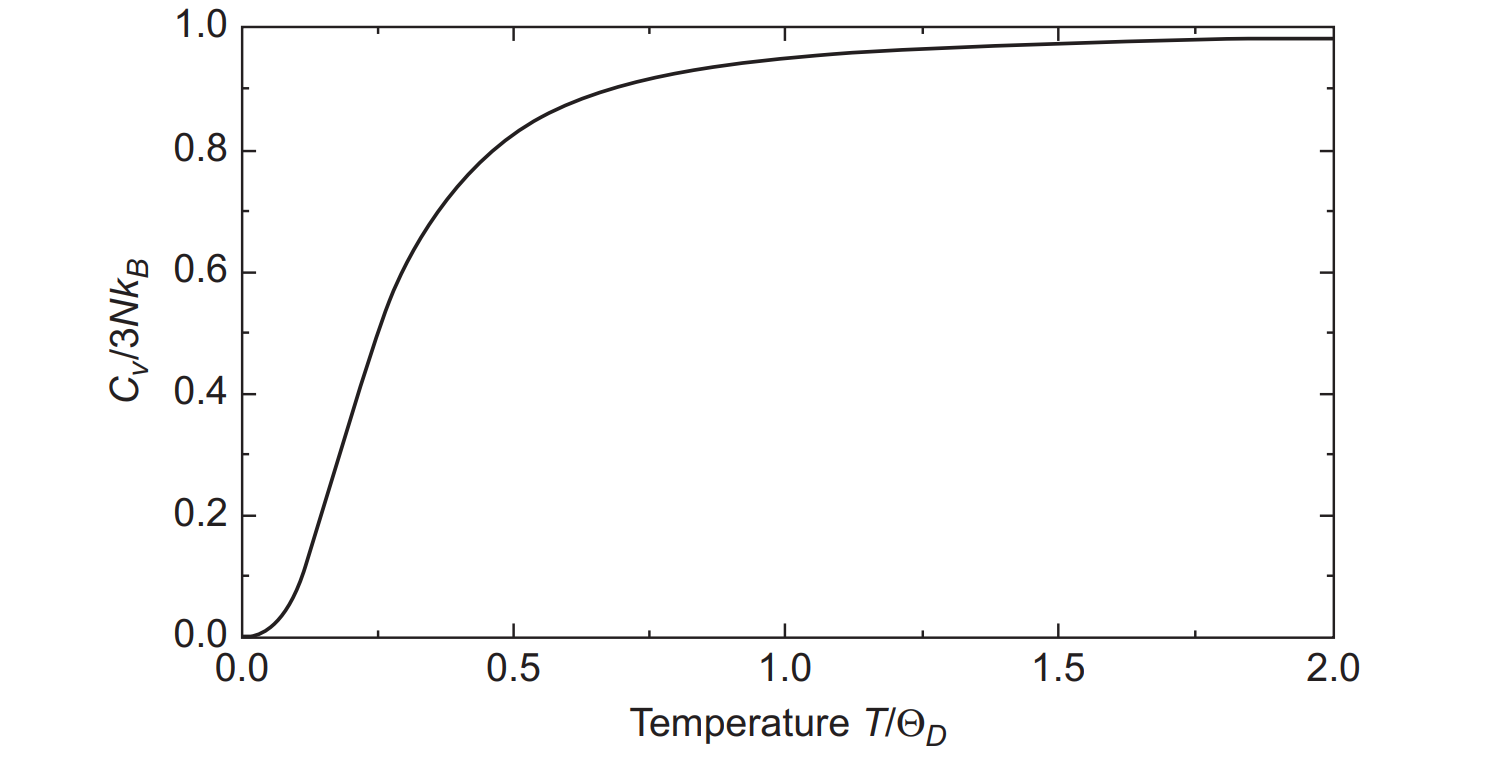
\includegraphics[width=0.8\textwidth]{fig/specific heat.png}
       \caption{晶体热容和温度的关系 \protect\footnotemark }
       \label{fig:specific heat with T}
\end{figure}
\footnotetext{图片来自Physics of Condensed Matter, P.K. Misra}

我们将用声子来描述机械波,声子和上文讨论的光子都是玻色子,区别在于\begin{enumerate}
    \item 作为弹性介质中的机械振动,其频率存在上限(由于力学的限制);
    \item 与光波一定是横波不同,机械波也可以是纵波。
\end{enumerate}

现在我们考虑一个$N$个原子的体系,其具有$3N$个自由度,将势能在极小值点$\diffp{U}{{x_i}}=0$的附近展开,有\begin{equation}
    U=U_0 =\frac{1}{2} \sum_{i=1}^{3N} \sum_{j=1}^N \diffp*{U}{{x_i}{x_j}}{0} \delta x_i \delta x_j=\frac{1}{2} \sum_{i,j} k_{ij} x_i x_j
\end{equation}
体系的动能可以写作\begin{equation}
    T=\frac{1}{2} \sum_{i=1}^{3N} \frac{p_i^2}{m_i}
\end{equation}
于是体系的哈密顿量为\begin{equation}
\begin{aligned}
    H&=T+V = \frac{1}{2} \sum_{i=1}^{3N} \frac{p_i^2}{m_i} +\frac{1}{2} \sum_{i,j} k_{ij} x_i x_j\\
    &=\frac{1}{2} \bd{p}^T M \bd{p} +\frac{1}{2}\bd{x}^T K \bd{x}
\end{aligned}
\end{equation}
其中\begin{equation}
    \bd{p}_{3N} =\begin{pmatrix}
        p_1\\
        p_2\\
        \vdots\\
        p_{3N}
    \end{pmatrix},\quad\bd{x}_{3N} =\begin{pmatrix}
        x_1\\
        x_2\\
        \vdots\\
        x_{3N}
    \end{pmatrix},\quad M= \begin{pmatrix}
        \frac{1}{m_1} & & \\
        & \ddots & \\
        & & \frac{1}{m_N}
    \end{pmatrix}_{3N\times 3N},\quad K= \begin{pmatrix}
        k_{1,1} & \cdots &k_{1,3N}\\
        \vdots & \ddots & \vdots\\
        k_{3N,1} & \cdots & K_{3N,3N}
    \end{pmatrix}
\end{equation}
其中$M$是一个对角阵,$K$是一个实对称方阵,它们一般无法同时直接对角化。采用质量权重变换:\begin{equation}
    \widetilde{p}_i = \frac{p_i}{\sqrt{m_i}} ,\quad \widetilde{x}_i =\sqrt{m_i} x_i,\quad[\widetilde{x}_i,\widetilde{p}_i]=i\hbar \delta_{ij},\quad \widetilde{k}_{ij} =\frac{k_{ij}}{\sqrt{m_i,m_j}}
\end{equation}
于是\begin{equation}
    H=\frac{1}{2} \bd{p}^T \cdot \bd{p}+\frac{1}{2} \widetilde{\bd{x}}^T\widetilde{K} \widetilde{\bd{x}}
\end{equation}
这个时候,存在$S^T S=1$满足,\begin{equation}
    S^T \widetilde{K} S=\Lambda
\end{equation}
其中$\Lambda=\mathrm{diag}(\lambda_1,\lambda_2,\cdots,\lambda_{3N})$
设\begin{equation}
    \widetilde{\bd{x}}=SQ,\quad \widetilde{\bd{p}}=SP
\end{equation}
从而得到\begin{equation}
\begin{aligned}
    H&=\frac{1}{2}\bd{p}^T \cdot \bd{p} +\frac{1}{2}Q^T \Lambda Q\\
    &=\sum_{i=1}^{3N} \left(p_k^2 +\lambda_k Q_k^2\right)\\
    &=\sum_{i=1}^{3N} h_k    
\end{aligned}
\end{equation}
其中$h_k=\frac{1}{2}(p_k^2+\lambda_k Q_k^2),\,\lambda_k=\omega_k^2\ge 0$。所以体系的哈密顿量可以分解为$3N$个部分,每个部分都是一个简谐振动。

对于每一个简谐振子,其能级分布为\begin{equation}
    \varepsilon_k(n_k)=(n_k+\frac{1}{2}) \hbar \omega_k
\end{equation}
我们可以将体系看作大量的声子组成的气体(phonon gas),每一个声子有$3N$种状态,第$k$个态的能量为$\varepsilon_k=\hbar \omega_k$,声子是一种玻色子,第$k$个态的占据数为$n_k$。

和光子气类似,声子也是全同粒子,并且总数不可确定,即其化学势是无意义的($\mu=0$)。类似地,我们可以将某一个微观态看作一组占据数:\begin{equation}
    v \leftrightarrow \{n_k\}
\end{equation}
每个状态对应的能量为\begin{equation}
    E_v =\sum_k (n_k +\frac{1}{2}) \hbar \omega_k
\end{equation}

我们可以对$3N$个可以区分的谐振子使用正则配分函数:\begin{equation}
    Q=\sum_v e^{-\beta E_v} =\prod_k Q_k
\end{equation}
其中$Q_k$是单谐振子配分函数,满足\begin{equation}
    Q_k =\sum_{n_k=0}^{\infty} e^{-\beta (n_k +\frac{1}{2})\hbar \omega_k} =\frac{e^{-\frac{1}{2}\beta \hbar \omega_k}}{1-e^{-\frac{1}{2}\beta \hbar \omega_k}}
\end{equation}

因此\begin{equation}
    \ln Q=\sum_k \ln \frac{e^{-\frac{1}{2}\beta \hbar \omega_k}}{1-e^{-\beta \hbar \omega_k}};
\end{equation}
根据正则系综中的结论:\begin{gather}
    \braket{E} =-\diffp{\ln Q}{\beta} =\sum_k \braket{\varepsilon_k(\omega_k)}    
\end{gather}
其中\begin{equation}
    \braket{\varepsilon_k(\omega_k)} =-\diffp{{\ln Q_k}}{\beta} =\frac{1}{2}\hbar \omega_k +\frac{1}{e^{\beta \hbar \omega_k}-1} \hbar \omega_k=(\braket{n_k}+\frac{1}{2}) \hbar \omega_k
\end{equation}

对于热容,我们有\begin{equation}
    C_V =\diffp{{\braket{E}}}{T} =\sum_k C_{V,k}
\end{equation}
其中\begin{equation}
\begin{aligned}
    C_{V,k}& =\diffp{\braket{\varepsilon_k}}{T} =-\frac{1}{k_B T^2} \diffp{\braket{\varepsilon_k}}{\beta}\\
    & =-\frac{\hbar\omega_k}{k_B T^2} \frac{-\hbar\omega_k e^{\beta\hbar\omega_k} }{\left(e^{\beta\hbar\omega_k}-1\right)^2}\\
    &=k_B (\beta\hbar\omega_k)^2 \frac{e^{\beta \hbar \omega_k}}{\left(e^{\beta\hbar\omega_k}-1\right)^2}
\end{aligned}
\end{equation}
记$\displaystyle \theta_k =\frac{\hbar \omega_k}{k_B}$,称为该振动模的振动特征温度\index{振动特征温度}。则有$\displaystyle \beta \hbar \omega_k=\frac{\theta_k}{T}$\begin{equation}
    C_{V,k} =k_B \left(\frac{\theta_k}{T}\right)^2 \frac{e^{\frac{\theta_k}{T}}}{(e^{\frac{\theta_k}{T}}-1)^2}
\end{equation}
不难发现$T\to+\infty$的时候,$C_{V,k}\to k_B$。

整个系统的热容,满足\begin{equation}
    C_V =\sum_k C_{V,k} =\int_0^{\omega_D} \di \omega g(\omega)C_V(\omega)
\end{equation}

类似前面的分析,在波矢空间中有\begin{equation}
    \rho(k)\di k =\frac{V}{2\pi^2} k^2 \di k
\end{equation}
并且$k=\frac{\omega}{c}$,注意到这个时候有两个横波自由度和一个纵波自由度\begin{equation}
    g(\omega)\di \omega =\frac{V}{2\pi^2} \left(\frac2{c_t^3}+\frac1{c_l^3}\right)\omega^2 \di \omega=A\omega^2 \di \omega
\end{equation}
我们知道有$3N$个简正模,因此\begin{equation}
    3N =\int_0^{\omega_D} g(\omega)\di \omega =\frac{1}{3}A \omega_D^3
\end{equation}
所以有$\displaystyle A=\frac{9N}{\omega_D^3}$。进而我们就可以计算热容\begin{equation}
    C_V =\int_0^{\omega_D} A\omega^2 k_B \left(\frac{\hbar\omega}{k_BT}\right)^2 \frac{e^{\frac{\hbar\omega}{k_BT}}}{\left(e^{\beta\hbar\omega_k}-1\right)^2}\di \omega^2
\end{equation}
做一个变量代换$\displaystyle x=\frac{\theta_k}{T}$就可以得到\begin{equation}
    C_V =9N k_B  \left(\frac{\hbar\omega_D}{k_BT}\right)^{-3}\int_0^{ \frac{\hbar\omega_D}{k_BT}} x^4 \frac{e^x}{(e^x-1)^2} \di x 
\end{equation}
令$\theta_D =\frac{\hbar\omega_D}{k_B}$。对于高温情形,$T\gg \theta_k$,所以$x\ll 1$,这个时候\begin{equation}
    C_V =9N k_B \left(\frac{\hbar\omega_D}{k_BT}\right)^{-3}\int_0^{ \frac{\theta_D}{T}}x^2 \di x  = 3N k_B 
\end{equation}

对于低温情形,$T\to 0$,$\theta_D\to \infty$,由\begin{equation}
    \int_{0}^{+\infty}\frac{x^4e^x}{(e^x-1)^2} \mathrm{d}x = \frac{4\pi^4}{15}
\end{equation}
所以\begin{equation}
    C_V =\frac{12}{5}\pi^4 N K_B \left(\frac{T}{\theta_D}\right)^3 \propto T^3 \label{equ:C_V in crystal}
\end{equation}

于是,我们就基本上解释了图\ref{fig:specific heat with T}所反映的物理现象。
% subsection 声子 (end)
% section photon_and_phonon (end)
\section{经典理想气体} % (fold)
\label{sec:经典理想气体}
\subsection{平动拆分} % (fold)
\label{sec:平动拆分}
事实上,单粒子的配分函数还可以进一步因子化,最常见的做法就是将平动的能级拆分出来\begin{equation}
    \varepsilon=\varepsilon_t+\varepsilon_{in}\Rightarrow q=q_t\cdot q_{in}
\end{equation}
其中$\varepsilon_t$和$q_t$是平动部分,$\varepsilon_{in}$和$q_{in}$是内部能量部分,进一步地,内部能量可以被拆分为核部分和其他部分(包括电子、振动、转动等)。即有\begin{equation}
    q=q_t q_n q_{\mathrm{other}}
\end{equation}
于是总的正则配分函数为\begin{equation}
\begin{aligned}
    \ln Q& = N \ln\frac{q}{N} +N\\
    & =\boxed{ N\ln \frac{q_t}{N}+N }+N \ln q_n + N \ln q_{\mathrm{other}}
\end{aligned}
\end{equation}
其中框内的部分都看作平动部分,框外的部分是分子内部结构的贡献。
% subsection 平动拆分 (end)
\subsection{无结构经典理想气体} % (fold)
\label{sub:无结构经典理想气体}
当气体分子没有内部结构的时候,只需要考虑平动的贡献。三维势箱中的一个粒子满足\begin{equation}
    \varepsilon(n_x,n_y,n_z)=\frac{h^2}{8mL^2} (n_x^2+n_y^2+n_z^2),\quad n_x,n_y,n_z=1,2,...
\end{equation}
某一个能级的态密度为\begin{equation}
    g(\varepsilon)\di \varepsilon =\frac{V}{4\pi^2}\cdot \frac{(2m)^{3/2}}{\hbar^3} \varepsilon^{1/2}\di \varepsilon
\end{equation}

从而平动配分函数为\begin{equation}
    q_t = \sum_i e^{-\beta \varepsilon_i} =\int_{0}^{+\infty} \rho(\varepsilon) e^{-\beta\varepsilon} \mathrm{d}x= \left(\frac{2\pi m k T}{h^2}\right)^{3/2} V =\frac{V}{\lambda^3}
\end{equation}

\begin{definition}
    上式中$\displaystyle \lambda=\sqrt{\frac{h^2}{2\pi m k T}}$被称为热波长\index{热波长}(Thermal wave length)。
\end{definition}
% subsection 无结构经典理想气体 (end)
\subsection{单原子和双原子理想气体分子} % (fold)
\label{sub:单原子和双原子理想气体分子}
\subsubsection{电子与核运动的分离}
对于单原子分子,原子内部的贡献仅限于核和电子。一个单原子分子的配分函数为\begin{equation}
    q=q_t q_n q_e
\end{equation}
其中原子核的部分可以写作$q_n=g_n^{(0)}e^{-\beta \varepsilon^{(0)}}=2I +1$,$I$是原子核的总自旋量子数。电子的部分可以写作\begin{equation}
\begin{aligned}
    q_e &=g_0^{(e)} e^{-\beta \varepsilon_0^{(e)}}+g_1^{(e)} e^{-\beta \varepsilon_1^{(e)}}+\cdots \\
    &=    e^{-\beta \varepsilon_0^{(e)}}\left(g_0^{(e)}+g_1^{(e)} e^{-\beta \delta \varepsilon_{10}^{(e)}}+\cdots\right)
\end{aligned}
\end{equation}
其中$\varepsilon_{j0}^{(e)}$是电子激发能,$g_j^{(e)}=2J+1$,$J$是该电子态的总角动量量子数。

在处理双原子分子的时候,我们首先需要假设核与电子的运动可以分离(这个近似被称为波恩-奥本海默近似\index{波恩奥本海默近似}或者绝热近似\index{绝热近似}):因为电子的运动速度比原子核快非常多,对于每一个电子态,可以认为核近似不动,对于原子核,可以认为电子形成了一个稳定的势场。

核的哈密顿量可以写成\begin{equation}
    H= K+V(R)
\end{equation}
其中动能$K=\frac{1}{2}(m_1 \dot{\bd{r}}_1^2 +m_2 \dot{\bd{r}}_2^2)$,在质心系中可以写成$K =\frac{1}{2}(M \dot{\bd{r}}_c^2 +\mu \dot{\bd{r}}^2)$。$\frac{1}{2}M \dot{\bd{r}}_c^2$的贡献纳入平动配分函数,因此核的哈密顿量只需要考虑相对运动项\begin{equation}
    \dot{\bd{r}}^2 =\dot{R}^2 + R^2 \dot\theta^2 +R^2 \sin^2\theta \dot\varphi^2
\end{equation}
所以\begin{equation}
    K=\frac{1}{2}\mu \left(\dot{R}^2 + R^2 \dot\theta^2 +R^2 \sin^2\theta \dot\varphi^2\right)
\end{equation}

\subsubsection{状态拆分}

双原子分子的配分函数可以拆分成核的贡献、分子内部结构的贡献和平动项的贡献。其中分子内部的贡献又可以进一步拆分成电子项、振动项和转动项。

我们对分子做完全解耦处理之后,配分函数就可以直接因子化。当电子的基态非常稳定的时候$\beta\Delta \varepsilon_{10}^{(e)}\gg 1$,所以\begin{equation}
    q_e\approx g_0^{(e)} e^{-\beta \varepsilon_0^{(e)}}
\end{equation}
对总配分函数的贡献只有一个因子,所以可以独立出来,即\begin{equation}
    q_{evr}=q_e q_{vr}
\end{equation}

\subsubsection{振动配分函数\index{振动配分函数}}
在声子气体中,\begin{equation}
    q_v =\frac{e^{-\beta \hbar \omega/2}}{1-e^{-\beta \hbar \omega}}=\frac{e^{-\frac12\frac{\theta_v}T}}{1-e^{-\frac{\theta_v}{T}}} =\begin{cases}
        \frac{T}{\theta_v}, & T\gg \theta_v\\
        e^{-\frac{\theta_v}{2T}},& T\ll \theta_v
    \end{cases}
\end{equation}
其中$\displaystyle \theta_v = \frac{\hbar\omega}{k_B}$被称为振动特征温度\index{振动特征温度},一般较大。而$\omega =\sqrt{\frac{k}{\mu}},k=\diffp*{U}{{R^2}}{0}$。
\subsubsection{转动配分函数\index{转动配分函数}}
对于一个刚性转子,我们有\begin{equation}
    \varepsilon_J = J(J+1)\frac{\hbar^2}{2I},\quad J=0,1,2,...,\ g_J=2J+1
\end{equation}
于是转动项对应的配分函数为\begin{equation}
    \begin{aligned}
        q_r &= \sum_{J=0}^{+\infty} (2J+1) e^{-J(J+1)\frac{\hbar^2}{2Ik_BT}}\\
        &= \sum_{J=0}^{+\infty} (2J+1) e^{-J(J+1)\frac{\theta_r}{T}}
    \end{aligned}
\end{equation}
其中$\displaystyle \theta_r=\frac{\hbar^2}{2I k_B}$被称为转动特征温度\index{转动特征温度},一般来说$\theta_r$比较小,可以作$\theta_r\ll T$近似。于是我们可以将求和转换成积分\begin{equation}
    q_r=\int_{0}^{+\infty} -\frac{T}{\theta_r}  \mathrm{d} e^{-J(J+1)\frac{\theta_r}{T}}=\frac{T}{\theta_r}
\end{equation}

\subsubsection{总配分函数}

综上,我们就得到了解耦近似下的所有配分函数,总配分函数为\begin{equation}
    q=\frac{q_n q_e q_t q_r q_v}{\sigma_{AB}}
\end{equation}
其中$\sigma$来自于经典的对称性或者量子力学熵的全同性原理,一般来说\begin{equation}
    \sigma_{AB} =\begin{cases}
        1 & A\neq B\\
        2 & A=B
    \end{cases}
\end{equation}
% subsection 单原子和双原子理想气体分子 (end)

\subsection{多原子分子气体} % (fold)
\label{sub:多原子分子气体}
多原子分子和双原子分子的分析方法是完全一致的,但是其自由度和配分函数会有一些不同。$N$原子分子会有$3N$个自由度,其中有三个平动自由度,线性分子有两个转动自由度,而非线性分子有三个转动自由度,剩下的自由度都属于振动自由度。
% subsection 多原子分子气体 (end)
% section 经典理想气体 (end)
\begin{review}
    \item 光的波粒二象性和黑体辐射;
    \item 声子和晶体的热容;
    \item 经典理想气体的平动拆分;
    \item 波恩奥本海默近似;
    \item 双原子分子的振动和转动配分函数;
\end{review}
\section{习题} % (fold)
\label{sec:习题5}

% section 习题 (end)
% chapter particles II (Application) (end)
%---------------------------------------------------------------------------
%---------------------------------------------------------------------------
\chapter{半导体} % (fold)
\label{cha:半导体}
\section{Intrinsic Semiconductor \& Extrinsic Semiconductor} % (fold)
\label{sec:Intrinsic Semiconductor and Extrinsic Semiconductor}
将Fermi-Dirac分布应用于半导体极大地推动了半导的研究和设计。
% section Intrinsic Semiconductor & Extrinsic Semiconductor (end)
\section{PN Junction} % (fold)
\label{sec:PN Junction}
% section PN Junction (end)
\section{Non-equilibrium Semiconductor} % (fold)
\label{sec:Non-equilibrium Semiconductor}
% section Non-equilibrium Semiconductor (end)
% chapter 半导体 (end)
%---------------------------------------------------------------------------
\chapter{气相化学平衡} % (fold)
\label{cha:气相化学平衡}
\section{导言} % (fold)
\label{sec:导言 9}
本章我们主要来处理理想气体的气相反应问题。基本思路是通过单粒子的配分函数$q$,获得反应的平衡常数$K$,从平衡常数可以进一步得到有关反应的热力学参数$\Delta_r G_m$、$\Delta_r H_m$、$\Delta_r S_m$等。
% section 导言 (end)
\section{具体分析} % (fold)
\label{sec:具体分析}
考察一个一般的气相化学反应:
\begin{equation*}
    \ce{a A + b B <=> c C + d D}
\end{equation*}
或者可以写成通式\begin{equation*}
    \sum_B v_B B =0
\end{equation*}

当体系达到化学平衡的时候,有\begin{equation}
    \sum_Bv_B \mu_B=0 \label{equ:equilibrium condition}
\end{equation}

对整体的配分函数进行因子化处理\begin{equation*}
    Q=\prod_B \frac{q_B^{N_B}}{N_B!}
\end{equation*}

根据我们前面得到的结论:\begin{align}
    A&=-kT \ln Q\\
    \mu_B &=\diffp*{A}{{N_B}}{T,V,\{n_C,C\neq B\}}
\end{align}
由此可以得到\begin{gather}
    A=-kT \sum_B \ln \frac{q_B^{N_B}}{N_B!}=-kT \sum_C \left[N_C\ln\frac{q_C}{N_C}+N_C\right]\\
    \mu_B =\diffp*{A}{{N_B}}{T,V,\{n_C,C\neq B\}}=-kT \ln \frac{q_B}{N_B}
\end{gather}
代入化学平衡条件\eqref{equ:equilibrium condition},可以得到\begin{equation}
    \sum_B v_B \ln \frac{q_B}{N_B}=0\Rightarrow \sum_B \ln q_B^{v_B} =\sum_B \ln N_B^{v_B}
\end{equation}

稍加变形,就有\begin{equation}
    \prod_B \frac{q_B^{v_B}}{V^{v_B}}=\prod_B \frac{N_B^{v_B}}{V^{v_B}}
\end{equation}
记数密度\begin{equation}
    \rho_B = \frac{N_B}{V}=\frac{p_B}{kT}
\end{equation}

于是\begin{equation}
    \begin{aligned}
        RHS.&=\prod_B \rho_B^{v_B} =\left(\prod_B \left(\frac{p_B}{p^{\ominus}}\right)^{v_B}\right) \cdot \left(\frac{p^\ominus}{kT}\right)^{\Delta v_B}\\
        &=K_p^\ominus \cdot \left(\frac{p^\ominus}{kT}\right)^{\Delta v_B}
    \end{aligned}
\end{equation}
而\begin{equation}
    LHS.=\prod_B \left(\frac{q_B(\text{in})}{\lambda_B^3}\right)^{v_B}
\end{equation}
其中$\lambda$为热运动波长,因为\begin{equation}
    q_t =\frac{V}{\lambda^3}
\end{equation}这里相当于约去了平动部分。

因为$q_B(in)=q_B^{(n)}q_{evr,B}$,因为化学反应前后原子核不会发生变化,所以\begin{equation}
    \prod_B (q_B^{(n)})^{v_B} =1 
\end{equation}
因此就有\begin{equation}
    \prod_B \left(\frac{q_{evr,B}}{\lambda_B^3}\right)^{v_B}=K_p^{\ominus} \cdot \left(\frac{p^{\ominus}}{kT}\right)^{\Delta v_B}
\end{equation}
% section 具体分析 (end)
\section{Examples} % (fold)
\label{sec:Examples}
\subsection{\ce{Na}的双聚} % (fold)
\label{sub:Na的双聚}
我们先来看反应\ce{Na2 (g) <=> 2Na (g)},显然应该有\begin{equation}
\begin{aligned}
    K_p &= \frac{\left(q_{evr,\ce{Na}}/\lambda^3_{\ce{Na}}\right)^2}{q_{evr,\ce{Na2}}/\lambda_{\ce{Na2}}^3}\\
    &=\frac{\lambda_{\ce{Na2}}^3}{\lambda_{\ce{Na}}^6} \frac{[g_{e,\ce{Na}}^{(0)}]^2 \cdot e^{-\beta \cdot 2 \varepsilon_{e,\ce{Na}}^{(0)}}}{\frac{T}{2\theta_r} \frac{e^{-\beta\hbar\omega/2}}{e^{-\theta_v/T}} \cdot g_{e,\ce{Na2}}^{(0)} e^{-\beta \varepsilon_{e,\ce{Na2}}^{(0)}} }
\end{aligned}
\end{equation}  

对于\ce{Na}原子,其电子组态未\ce{[Ne]3s^1},因此$S=\frac{1}{2}$,因而$g_{e,\ce{Na}}^{(0)}=2$,而对于\ce{Na2},基态时$S=0$,因而$g_{e,\ce{Na2}}^{(0)}=1$。再考虑到热波长满足\begin{equation}
    \lambda_B =\sqrt{\frac{2\pi m_B kT}{h^2}}
\end{equation}
原式可以化简为\begin{equation}
    K_p=8 \left(\frac{\pi m_{\ce{Na}}kT}{h^2}\right)^{3/2} \frac{\theta_{r,\ce{Na2}}}{T} \left(1-e^{\frac{\theta_{v,\ce{Na2}}}{T}}\right)e^{-\beta D_0}
\end{equation}
其中\begin{equation}
    D_0 = 2\varepsilon_{e,\ce{Na}}^{(0)} -\varepsilon_{e,\ce{Na}}^{(0)}-\frac{1}{2}\hbar\omega
\end{equation}
% subsection \ce{Na}的双聚 (end)
\subsection{\ce{H2}和\ce{I2}反应} % (fold)
\label{sub:H2和I2反应}
我们再来看反应\ce{H2 + I2 <=> 2HI},类似上面的结果,我们有\begin{equation}
    \begin{aligned}
        K_p& = \frac{q_{evr,\ce{HI}}}{q_{evr,\ce{H2}}q_{evr,\ce{I2}}} \cdot \frac{\lambda_{\ce{H2}}^3\lambda_{\ce{I2}}^3}{\lambda_{\ce{HI}}^6}\\
        &= \frac{m_{\ce{HI}}}{m_{\ce{H2}^{3/2}}\cdot m_{\ce{I2}^{3/2}}}\cdot \frac{4\theta_{r,\ce{H2} }\theta_{r,\ce{I2}}}{\theta_{r,\ce{H2}}^2} \cdot \frac{\left(1-e^{-\theta_v(\ce{H2})/T}\right)\left(1-e^{-\theta_v(\ce{I2})/T}\right)}{\left(1-e^{-\theta_v(\ce{HI})/T}\right)^2} \cdot \frac{e^{\beta (2D_{e}^{\ce{HI}}-D_{e}^{\ce{H2}}-D_{e}^{\ce{I2}})}}{e^{\beta (2\cdot \frac{1}{2} \hbar \omega_{\ce{HI}}-\frac{1}{2}\hbar\omega_{\ce{H2}}-\frac{1}{2}\hbar\omega_{\ce{I2}})} }\\
        &=Ae^{\beta (2D_{e}^{\ce{HI}}-D_{e}^{\ce{H2}}-D_{e}^{\ce{I2}})}
    \end{aligned}
\end{equation}
% subsection \ce{H2}和\ce{I2}反应 (end)
% section Examples (end)

\begin{review}
    \item 化学平衡常数和分子配分函数的关系;
    \item \ce{Na}的双聚和\ce{H2}和\ce{I2}反应;
    \item 零点能校正
\end{review}
\section{习题} % (fold)
\label{sec:习题gas reaction}

% section 习题 (end)
% chapter 气相化学平衡 (end)
%---------------------------------------------------------------------------
\chapter{自由电子气} % (fold)
\label{cha:自由电子气}
\section{Introduction} % (fold)
\label{sec:Introduction 8}
电子是费米子,由于Pauli不相容原理,宏观量级的电子最终会排布到很高的能级上,这个能级我们就称之为费米能级\index{费米能级}。

金属中的自由电子我们依旧使用真空电子势箱模型来描述,因此电子的各个能级也就是真空势箱中自由粒子的平动能级。所以费米能级附近的粒子实际上具有相当高的动能。由于这些粒子的动能很大,电子和正离子、电子和电子之间的相互作用势能可以忽略,所以我们可以近似看出自由电子气。
% section Introduction (end)
\section{统计分析} % (fold)
\label{sec:统计分析}
对于费米子,我们使用Fermi-Dirac分布$f(\mu)$来描述其能量分布,这个分布函数的大概图像为
\begin{figure}[h]
       \centering
       \subfigure[正常温度情形]{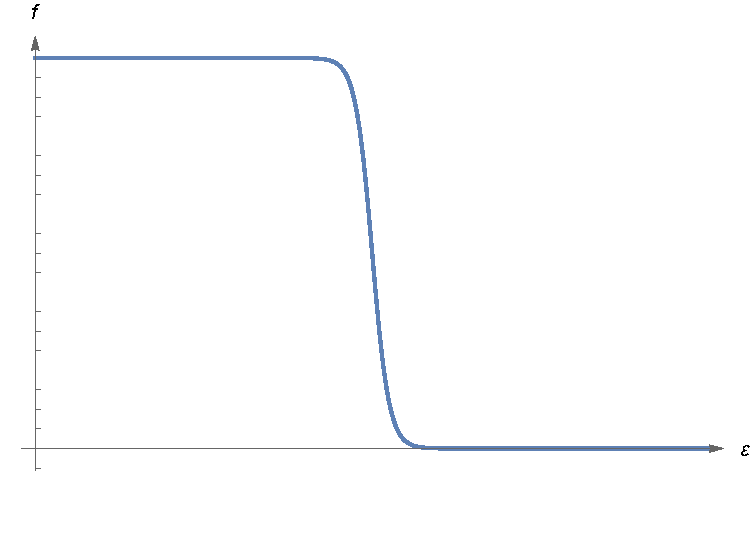
\includegraphics[width=0.42\textwidth]{fig/Fermi distribution.pdf}}\qquad
       \subfigure[低温情形]{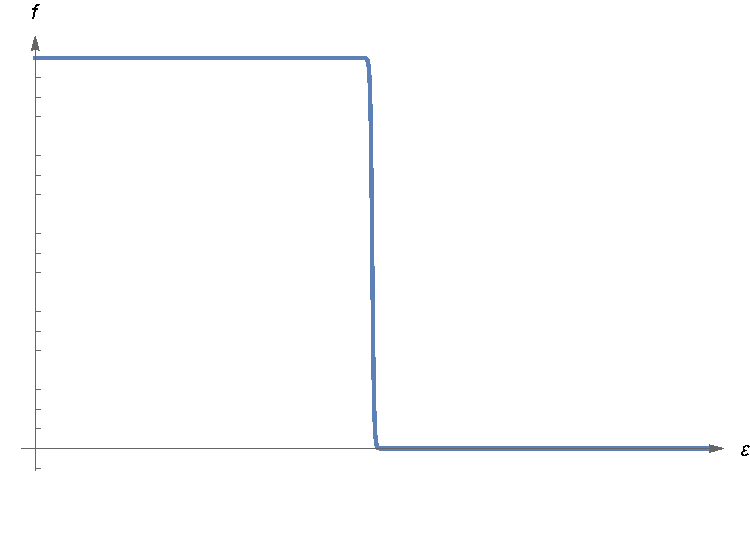
\includegraphics[width=0.42\textwidth]{fig/sharp fermidis.pdf}}
       \caption{Fermi-Dirac分布的大概图像}
       \label{fig:fermi distribution}
\end{figure}
而不同能级的总粒子数量满足满足关系\begin{equation}
    N(\varepsilon) = C \sqrt{\varepsilon} f(\varepsilon) 
\end{equation}
其图像为
\begin{figure}[h]
    \centering
    \subfigure[正常温度情形]{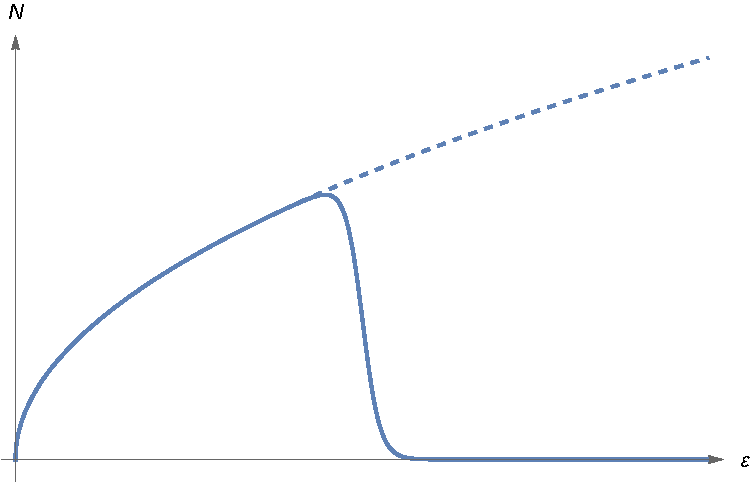
\includegraphics[width=0.42\textwidth]{fig/LowTempNum.pdf}}\qquad
    \subfigure[低温情形]{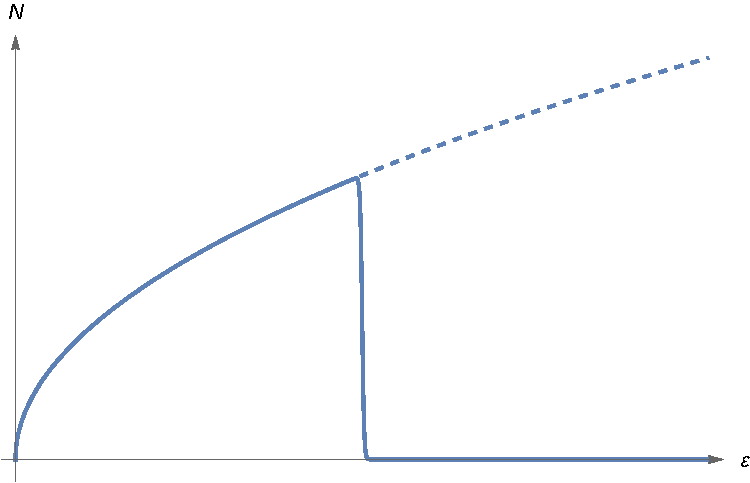
\includegraphics[width=0.42\textwidth]{fig/HighTempNum.pdf}}
    \caption{不同能级的粒子总数}
    \label{fig:fermi distribution times sqrte}
\end{figure}

记$x=\beta(\varepsilon-\mu)$,就有\begin{equation}
    f(x)'=\frac{e^x}{(e^x+1)^2}=\frac{1}{(1+e^x)(1-e^{-x})}
\end{equation}
利用巨正则系综中的结论\begin{equation}
    \beta p V =\ln \Xi =\sum_j g_j \ln (1+ e^{\beta (\mu-\varepsilon_j)}) \di \varepsilon
\end{equation}
对能级的求和可以化为对平动动能的积分\begin{equation}
    \ln \Xi =2 \int_0^\infty \rho(\varepsilon) \ln (1+e^{\beta (\mu-\varepsilon) })
\end{equation}
考虑到\begin{gather}
    \braket{N} = \sum_i \braket{n_i} =2 \int_{0}^{+\infty} \rho(\varepsilon) f(\varepsilon) \mathrm{d}\varepsilon\\
    \braket{E} =\sum_i \braket{n_i} \varepsilon_i =2\int_{0}^{+\infty} \rho(\varepsilon)f(\varepsilon) \varepsilon\mathrm{d}\varepsilon
\end{gather}

前面我们已经给出了\begin{equation}
    \rho(\varepsilon) \di\varepsilon =\frac{2\pi V}{h^3} (2m)^{3/2} \varepsilon^{1/2}\di \varepsilon
\end{equation}
\subsection{0K的情形} % (fold)
\label{sub:0K的情形}
这个时候电子只会占据$0\sim \mu_0$的能级,\begin{equation}
    f(\varepsilon)=\begin{cases}
        1 & \varepsilon <\mu_0\\
        0 & \varepsilon>\mu_0
    \end{cases}
\end{equation}
于是我们就有\begin{equation}
    \braket{N}=\int_0^{\mu_0} \frac{4\pi V }{h^3} (2m)^{3/2} \varepsilon^{1/2}\di \varepsilon =\frac{8\pi V}{3h^3} (2m)^{3/2} \mu_0^{3/2} \label{equ:N with E fermi}
\end{equation}
\begin{definition}
    我们称$T_F$满足\begin{equation}
        \mu_0 =k_B T_F
    \end{equation}
    为费米温度\index{费米温度}。
\end{definition}

\begin{example}
    常温下铜的密度为8.960g/cm³,尝试求铜的费米能级和费米温度。
\end{example}
\begin{solution}
    由式\eqref{equ:N with E fermi}可以得到\begin{equation}
        \mu_0 =(\frac{3h^3 \braket{N}}{8\pi V})^{2/3}/2m =1.0602\times 10^{-17} \mathrm{J}
    \end{equation}
    其费米温度为\begin{equation}
        T_F =\mu_F/k_B=7.68\times 10^5 \mathrm{K}
    \end{equation}
\end{solution}

平均能量满足\begin{equation}
    \begin{aligned}
        \braket{E} &= \int_0^{\mu_0} \frac{4\pi V}{h^3} (2m)^{2/3} \varepsilon^{3/2} \di \varepsilon\\
        &=\frac{2}{5} \frac{4\pi V}{h^3} (2m)^{2/3} \mu_0^{5/2}\\
        &=\frac{3}{5} \braket{N}\mu_0 =\frac{3}{5} \braket{N} k_B T_F
    \end{aligned}
\end{equation}
% subsection 0K的情形 (end)
\subsection{非0K的情形} % (fold)
\label{sub:非0K的情形}
一般地,我们有\begin{equation}
    \braket{E}= 2\int_{0}^{+\infty} \rho(\varepsilon) \varepsilon f(\varepsilon)
    \di \varepsilon 
\end{equation}
我们记\begin{equation}
    \varphi(\varepsilon) =2\int_0^\varepsilon \rho(\varepsilon') \varepsilon' \di \varepsilon'
\end{equation}
则$\displaystyle \di \varphi(\varepsilon) =\rho(\varepsilon) \varepsilon \di \varepsilon$,于是我们就有
\begin{equation}
    \begin{aligned}
        \braket{E}& =\int_0^\infty f(\varepsilon) \di \varphi(\varepsilon)\\
        &=\left. f(\varepsilon) \rho(\varepsilon) \right|_0^\infty -\int_{0}^{+\infty}\varphi(\varepsilon)f'(\varepsilon) \mathrm{d}\varepsilon
    \end{aligned}
\end{equation}
因为$\varepsilon\to+\infty$的时候和$\varepsilon\to 0$的时候$f(\varepsilon)\varphi(\varepsilon)$均趋于0,所以\begin{equation}
    \braket{E} = -\int_{0}^{+\infty}\varphi(\varepsilon)f'(\varepsilon) \mathrm{d}\varepsilon
\end{equation}
考虑到\begin{equation}
    f(\varepsilon)'=-\frac{\beta e^{\beta(\varepsilon-\mu)}}{(1+e^{\beta(\varepsilon-\mu)})^2}
\end{equation}
其大致图像为
\begin{figure}[h]
       \centering
       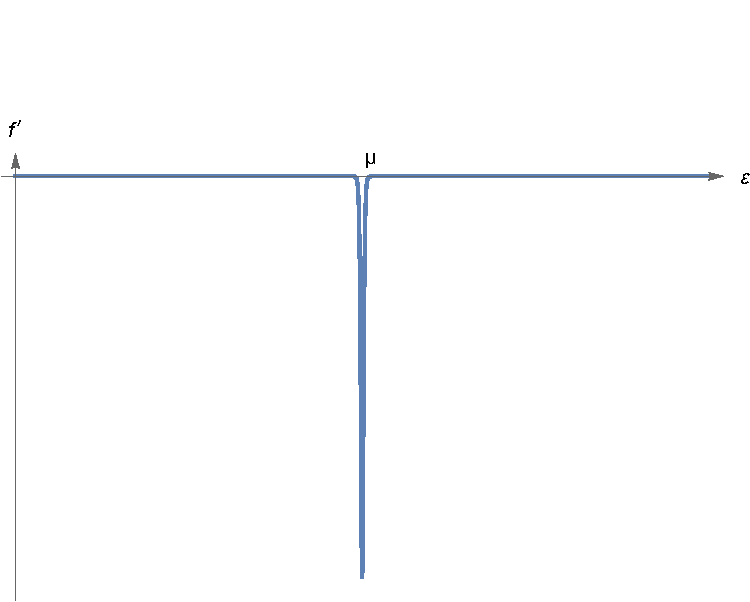
\includegraphics[width=0.5\textwidth]{fig/fermiD.pdf}
       \caption{$f'(\varepsilon)$函数}
       \label{fig:Dfermidistribution}
\end{figure}

所以\begin{equation}
    \braket{E} = -\int_{0}^{+\infty}\varphi(\varepsilon)f'(\varepsilon) \mathrm{d}\varepsilon \approx  -\int_{-\infty}^{+\infty}\varphi(\varepsilon)f'(\varepsilon) \mathrm{d}\varepsilon 
\end{equation}

我们将$\varphi(\varepsilon)$在$\varepsilon=\mu$的附近展开,因此就有\begin{equation}
    \varphi=\sum_{m=0}^\infty\left. \frac{\varphi^{(m)}(\varepsilon)}{m!}\right|_{\varepsilon=\mu}(\varepsilon-\mu)^m,\quad m=0,2,4,\cdots
\end{equation}

$m$取偶数是因为$f'(\varepsilon)$关于$\varepsilon-\mu$对称,因此奇数次项的积分为零。所以\begin{equation}
    \braket{E} =\sum_{m=0}^{\infty} \frac{\varphi^{(m)}(\mu)}{m!} \int_{-\infty}^{+\infty}(\varepsilon-\mu)^m [-f'(\varepsilon)] \mathrm{d}\varepsilon
\end{equation}
记$x=\beta(\varepsilon-\mu)$,我们记\begin{equation}
    L_m(x) = \int_{-\infty}^{+\infty}x^m/\beta^m [-f'(x)] \mathrm{d}\varepsilon=\frac{1}{\beta^m} \int_{-\infty}^{+\infty}\frac{x^m }{(1+e^x)(1+e^{-x})}\mathrm{d}\varepsilon 
\end{equation}
其中\[L_0 =1, \quad L_2=\frac{\pi^2}{3} (kT)^2,\quad L_4 =\frac{7\pi^4}{15} (kT)^4 \]
所以\begin{equation}
    \braket{E} =\sum_{m=0}^{\infty}L_m \frac{\varphi^{(m)}(\mu)}{m!}
\end{equation}

现在关键的问题是这个时候的$\mu$,为了求解这个$\mu$,我们首先求解$\braket{N}$,注意到\begin{equation}
    \braket{N} = 2  \int_{0}^{+\infty} \rho(\varepsilon) f(\varepsilon)\mathrm{d}\varepsilon 
\end{equation}
类似地,记$g(\varepsilon)=2\int_0^\varepsilon \di \varepsilon' \rho(\varepsilon')$,于是就有\begin{equation}
    \braket{N} =\sum_{m=0}^{+\infty} L_m\frac{g^{(m)}(\mu)}{m!}
\end{equation}
其中\[g(\varepsilon) = \frac{8\pi V}{3h^3} (2m)^{3/2} \varepsilon^{3/2},\quad g^{(2)} (\varepsilon) =\frac{2\pi V}{h^3} (2m)^{3/2} \varepsilon^{-1/2},g^{(4)}(\varepsilon)=\frac{3\pi V}{2h^3} (2m)^{3/2}\varepsilon^{-5/2}\]

所以\begin{equation}
    \begin{aligned}
        \braket{N}&=\frac{8\pi V}{3h^3}(2m)^{3/2}  \mu^{3/2} +\frac{\pi V}{h^3}(2m)^{3/2} \mu^{-1/2} +\frac{\pi V}{16h^3} \mu^{-5/2} +\cdots\\
        &= \frac{8\pi V}{3h^3}(2m)^{3/2}  \mu^{3/2}\left[1+\frac
        {\pi^2}{8} \left(\frac{kT}{\mu}\right)^2+o\left(\frac{kT}{\mu}\right)^4\right]
    \end{aligned}
\end{equation}
由于$N$不会随着温度变化而变化,所以当$T=0$的时候\begin{equation}
    \braket{N} = \frac{8\pi V}{3h^3}(2m)^{3/2}  \mu_0^{3/2}
\end{equation}
所以\begin{equation}
    \mu=\mu_0\left[1+\frac
        {\pi^2}{8} \left(\frac{kT}{\mu_0}\right)^2+o\left(\frac{kT}{\mu_0}\right)^4\right]^{-2/3}
\end{equation}
当$T$比较小的时候,就有\begin{equation}
    \mu=\mu_0\left[1-\frac
        {\pi^2}{12} \left(\frac{kT}{\mu_0}\right)^2 +o\left(\frac{kT}{\mu_0}\right)^4\right]
\end{equation}
也即:随着温度的升高,化学势略有降低,但是下降的不多。

现在我们完成了$\mu$的求解,于是就有\begin{equation} 
    \braket{E} =\sum_{m=0}^{\infty}L_m \frac{\varphi^{(m)}(\mu)}{m!}
\end{equation}
因为\begin{equation}
    \begin{gathered}
        \varphi(\varepsilon)=\frac{4\pi V}{h^3} (2m)^{3/2}\int_0^\varepsilon {\varepsilon'}^{3/2} \mathrm{d}\varepsilon'= \frac{8\pi V}{5h^3} (2m)^{3/2} \varepsilon^{5/2}\\
        \varphi^{(2)}(\varepsilon)= \frac{6\pi V}{h^3} (2m)^{3/2} \varepsilon^{1/2},\quad
        \varphi^{(4)}(\varepsilon)= \frac{9\pi V}{2h^3} (2m)^{3/2} \varepsilon^{-3/2}
    \end{gathered}
\end{equation}
所以\begin{equation}
    \begin{aligned}
        \braket{E} &=\frac{8\pi V}{5h^3}(2m)^{3/2}  \mu^{5/2} +\frac{3\pi V}{h^3}(2m)^{3/2} \mu^{1/2} \frac{\pi^2}{3}(kT)^2+\frac{3\pi V}{16h^3} \mu^{-3/2} \frac{7\pi^4}{15}(kT)^2+\cdots\\
        &= \frac{8\pi V}{5h^3}(2m)^{3/2}  \mu^{5/2}\left[1+\frac
        {5\pi^2}{8} \left(\frac{kT}{\mu}\right)^2+o\left(\frac{kT}{\mu}\right)^4\right]\\
        &= \frac{8\pi V}{5h^3}(2m)^{3/2}  \mu_0^{5/2}\left[1-\frac
        {5\pi^2}{24} \left(\frac{kT}{\mu_0}\right)^2+o\left(\frac{kT}{\mu_0}\right)^4\right] \left[1+\frac{5\pi^2}{8}\left(\frac{kT}{\mu_0}\right)^2+o\left(\frac{kT}{\mu_0}\right)^4\right]\\
        & = \frac{8\pi V}{5h^3}(2m)^{3/2}  \mu_0^{5/2}\left[1+\frac
        {5\pi^2}{12} \left(\frac{kT}{\mu_0}\right)^2+o\left(\frac{kT}{\mu_0}\right)^4\right]\\
        & = \braket{E}_0 \left[1+\frac
        {5\pi^2}{12} \left(\frac{kT}{\mu_0}\right)^2+o\left(\frac{kT}{\mu_0}\right)^4\right]\\
        & =\frac{3}{5} Nk_B T_F \left[1+\frac
        {5\pi^2}{12} \left(\frac{kT}{\mu_0}\right)^2+o\left(\frac{kT}{\mu_0}\right)^4\right]
    \end{aligned}
\end{equation}

由此可以得到系统的热容为\begin{equation}
    C_V= \diffp*{{\braket{E}}}{T}{\, V} = \frac{3}{5} Nk_B T_F \frac{\pi^2}{12} \frac{2T}{T_F^2} +o(T^3) =\frac{\pi^2}{2} Nk_B \frac{T}{T_F}
\end{equation}
根据式\eqref{equ:C_V in crystal},晶体由晶格振动带来的热容为\begin{equation}
    C_V =\frac{12}{5}\pi^4 N K_B \left(\frac{T}{\theta_D}\right)^3 \propto T^3
\end{equation}
因为$T_F$很大,所以温度较高的时候,自由电子气的热容相比于晶格振动的热容要小很多。但是极低温度下,晶格热容$C_V \propto T^3$,此时自由电子气热容占主导。

% subsection 非0K的情形 (end)
% section 统计分析 (end)
\section{习题} % (fold)
\label{sec:习题8}

% section 习题 (end)
% chapter 自由电子气 (end)
%---------------------------------------------------------------------------
%---------------------------------------------------------------------------
\chapter{Bose-Einstein凝聚} % (fold)
\label{cha:Bose-Einstein凝聚}
\section{Introduction} % (fold)
\label{sec:Introduction 9}
对于无结构无内禀简并度的玻色子和费米子,我们有\begin{equation}
    \begin{aligned}
        \beta p V &=\ln \Xi_{\substack{FB\\BE}}= \int_{0}^{+\infty}\pm \left(1\pm e^{\beta(\mu-\varepsilon)}\right)  g(\varepsilon) \mathrm{d}\varepsilon\\
        &=2\pi V \left(\frac{m}{2\hbar^2 \pi^2}\right)^{3/2}\int_{0}^{+\infty} \pm \ln(1\pm e^{\beta(\mu-\varepsilon)}) \varepsilon \mathrm{d}\varepsilon
    \end{aligned}
\end{equation}
令$z=e^{\beta\mu},y=\beta \varepsilon$,于是\begin{equation}
    \beta p\Lambda_B^3 =\frac{4}{\sqrt{4}} \int_{0}^{+\infty} \pm \ln(1\pm ze^{-y})y^{1/2} \mathrm{d}y
\end{equation}
再令$y=x^2$,因此\begin{equation}
    \begin{aligned}
        \beta p\Lambda_B^3 &=\pm \frac{4}{\sqrt\pi} \int_{0}^{+\infty} \ln(1\pm ze^{-x^2})x^2 \mathrm{d}x\\
        &=\pm \frac{4}{\sqrt\pi} \int_{0}^{+\infty} \sum_{n=1}^{\infty}  (-1)^{n+1} \frac{(\pm1)^n z^n e^{-n x^2}}{n}x^2\mathrm{d}x\\
        & =(\mp)^{n+1} \sum_{n=1}^{+\infty} \frac{z^n}{n}  \int_{0}^{+\infty} e^{-n x^2}x^2\mathrm{d}x\\
        & = \sum_{n=1}^{+\infty}  \frac{(\mp)^{n+1} }{n^{5/2}} z^n 
    \end{aligned}
\end{equation}
即有\begin{equation}
    \beta p V = \frac{V}{\Lambda_B^3} \sum_{n=1}^{+\infty}  \frac{(\mp)^{n+1} }{n^{5/2}} z^n 
\end{equation}
对于费米子和玻色子就有\begin{equation}
    \ln \Xi_{\substack{FB\\BE}}=\frac{V}{\Lambda_B^3} \sum_{n=1}^{+\infty}  \frac{(\mp)^{n+1} }{n^{5/2}} z^n
\end{equation}
因此\begin{equation}
    \begin{aligned}
        \braket{E}&=-\diffp*{{\ln \Xi_{\substack{FB\\BE}}}}{\beta}{\, V,\zeta} =3 \ln \Xi_{\substack{FB\\BE}} \cdot \frac{1}{\Lambda_B} \diffp{\Lambda_B}{\beta}\\
        &=\frac{3}{2}k_B T\ln \Xi_{\substack{FB\\BE}} 
    \end{aligned}
\end{equation}
同时\begin{equation}
    \begin{aligned}
        \braket{N}_{\substack{FB\\BE}}&=-\diffp*{{\ln \Xi_{\substack{FB\\BE}}}}{{(-\beta\mu)}}{\, \beta, V} =\diffp{{\ln \Xi_{\substack{FB\\BE}}}}{z} \diffp{z}{{(\beta\mu)}} \\
        &= z \cdot \frac{V}{\Lambda_B^3} \sum_{n=1}^{\infty}\frac{(\mp 1)^{n+1}}{n^{3/2}} z^{n-1}\\
        &=\frac{V}{\Lambda_B^3} \sum_{n=1}^{\infty}\frac{(\mp 1)^{n+1}}{n^{3/2}} z^{n}\\
    \end{aligned}
\end{equation}

% section Introduction (end)
\section{Bose-Einstein凝聚} % (fold)
\label{sec:Bose-Einstein凝聚}
\begin{definition}
    当发生玻色-爱因斯坦凝聚\index{玻色-爱因斯坦凝聚}的时候,有宏观量级的玻色子处于$\varepsilon=0$的基态,i.e.\begin{equation}
        n\left(\epsilon_{s}\right) \equiv \lim _{V \rightarrow \infty} \frac{f\left(\epsilon_{s}\right)}{V}=\lim _{V \rightarrow \infty} \frac{1}{V} \frac{1}{\exp \left[\left(\epsilon_{s}-\mu\right) / \tau\right]-1} \neq 0.
    \end{equation}
\end{definition}
回顾我们之前的\begin{equation}
    \begin{aligned}
        \beta p V &=\ln \Xi_{\substack{FB\\BE}}= \int_{0}^{+\infty}\pm \left(1\pm e^{\beta(\mu-\varepsilon)}\right)  g(\varepsilon) \mathrm{d}\varepsilon\\
        &=2\pi V \left(\frac{m}{2\hbar^2 \pi^2}\right)^{3/2}\int_{0}^{+\infty} \pm \ln(1\pm e^{\beta(\mu-\varepsilon)}) \mathrm{d}\varepsilon
    \end{aligned}
\end{equation}
这里我们无意中忽略了$\varepsilon=0$的项,这在大多数情况下是没有问题的,因为$\displaystyle \int_{a}^{b}f(x) \mathrm{d} x =\int_{a}^{b}f(x)+g(x) \mathrm{d} x$,其中$g(x)$只在有限个点取有限的值。但是这里的$\varepsilon=0$的位置有宏观量级的粒子,反应在积分中就相当于在$\varepsilon=0$处出现了$\delta$函数。因此我们可以在原式中加上端点的值$-\ln(1-z)$,这将不会对原来的积分产生影响,因此\begin{equation}
    \beta p V=\ln \Xi=\frac{V}{\Lambda_B^3} \sum_{n=1}^{\infty}\frac{1}{n^{5/2}} z^{n}-\ln(1-z)
\end{equation}
于是我们就有\begin{equation}
    \braket{N}_{BE} = \frac{V}{\Lambda_B^3} \sum_{n=1}^{\infty}\frac{1}{n^{3/2}} z^{n}+\frac{z}{1-z} 
\end{equation}

于是当粒子数固定的时候,减小$T$或者$V$都会使基态占据数\begin{equation}
    n_0 = \frac{1}{e^{-\beta \mu}-1} = \frac{z}{1-z}
\end{equation}

\begin{definition}
    定义凝聚温度\index{凝聚温度}$T_c$满足\begin{equation}
        N(T_c) =\frac{V}{\Lambda_B^3} \sum_{n=1}^{\infty} \frac{1}{n^{3/2}} = V n_Q \zeta(\frac{3}{2}) = \frac{V}{h^3} (2\pi m k_B T_c)^{3/2} \zeta(3/2)
    \end{equation}
    其中$n_Q=\frac{1}{\Lambda_B^3}$被称为quantum density,上式也即\begin{equation}
        \frac{n(T_c)}{n_Q} =\zeta(\frac{3}{2})
    \end{equation}
    相应的$T_c$为\begin{equation}
        T_c = \left(\frac{N(T_c)}{v\zeta(3/2)}\right)^{2/3} \frac{h^2}{2\pi m k_B}
    \end{equation}
\end{definition}

当温度在凝聚温度以上的时候$n_0\ll N$,而当温度降到凝聚温度以下的时候,\begin{equation}
    N=\frac{V}{\Lambda_B^3} \zeta(3/2) +n_0=N \left(\frac{T}{T_c}\right)^{3/2} +n_0
\end{equation}
在凝聚温度以下,$n_0$逐渐增加到宏观量级。i.e.\begin{equation}
    \frac{n_0}{N} =1- \left(\frac{T}{T_c}\right)^{3/2}
\end{equation}

这个时候\begin{equation}
    \ln \Xi = \frac{V}{\Lambda_B^3}  \sum_{n=1}^{\infty} \frac{1}{n^{5/2}} -\ln(1-z) = \frac{V}{\Lambda_B^3}\zeta(5/2) -\ln(1-z)
\end{equation}

于是\begin{equation}
    \braket{E} =-\diffp{\ln \Xi}{\beta} = \frac{3V}{\Lambda_B^4}\zeta(5/2) \frac{h}{2\sqrt{2\pi mk_B T}} -\frac{\mu z}{z-1}
\end{equation}

% section Bose-Einstein凝聚 (end)
\section{Example:\ce{{}^4He}} % (fold)
\label{sec:Example:He 3}

% section Example:He 3 (end)
\begin{review}
    \item 无结构无内禀简并度的玻色子/费米子巨配分函数;
    \item Bose-Einstein凝聚的概念;
    \item Bose-Einstein凝聚的条件和凝聚温度;
    \item 凝聚态的热力学性质
    \item \ce{{}^4 He}的Bose-Einstein凝聚;
\end{review}

\section{习题} % (fold)
\label{sec:习题9}

% section 习题 (end)
% chapter Bose-Einstein凝聚 (end)
%---------------------------------------------------------------------------
\chapter{磁学系统的相变 I} % (fold)
\label{cha:磁学系统的相变 I}
\section{Introduction} % (fold)
\label{sec:Introduction}
\subsection{问题背景} % (fold)
\label{sub:问题背景}
前面我们所了解的统计力学,大多数处于下面的范式之中

\begin{enumerate}\setlength{\itemsep}{0pt}
    \item 首先计算体系的能谱,对于给定的某一个态$v$,求解$E_v$,$v$在经典力学中指的是相空间中的点,在量子力学中指的是离散的微观态。
    \item 然后计算配分函数,比如对于正则系综,有\begin{equation}
              Q=\sum_{v}e^{-\beta E_v}
          \end{equation}
    \item 最后利用热力学的有关理论关联到具体的宏观热力学性质。比如常见的热力学函数\begin{equation}
        F=-kT\ln Q\\
        \di F = -S\di T -p\di V +\mu \di N
    \end{equation}
\end{enumerate}

实际应用中,这一套理论存在两大问题:$E_v$求解困难;$Q$计算困难。此外,我们前面一段时间所讨论的系统都是无相互作用的,这个情况显然也是过于理想化的。从本章开始我们将致力于研究有相互作用的复杂体系。

相变\index{相变},就是显著的相互作用带来的结果。
% subsection 问题背景 (end)

\subsection{PVT系统和HMT系统} % (fold)
\label{sub:PVT系统和HMT系统}
本章中我们主要讨论磁学系统的相变,这个体系相对陌生,因此我们首先将其和我们较为熟悉的热力学系统的相变类比。
% subsection PVT系统和HMT系统 (end)
\subsection{Ising模型和磁学热力学} % (fold)
\label{sub:Ising模型和磁学热力学}

% subsection Ising模型和磁学热力学  (end)

% section Introduction (end)
\section{相变现象和Ising模型的解析解} % (fold)
\label{sec:相变现象和Ising模型的解析解}

% section 相变现象和Ising模型的解析解 (end)

% chapter 磁学系统的相变 I (end)
\chapter{磁学系统的相变 II} % (fold)
\label{cha:磁学系统的相变 II}
\section{关联函数} % (fold)
\label{sec:关联函数}

% section 关联函数 (end)
\section{平均场理论} % (fold)
\label{sec:平均场理论}

% section 平均场理论 (end)
\section{重整化群方法} % (fold)
\label{sec:重整化群方法}

% section 重整化群方法 (end)
% chapter 磁学系统的相变 II (end)
\chapter{相图} % (fold)
\label{cha:相图}
\section{van der Waals方程和气液相变} % (fold)
\label{sec:van der Waals方程和气液相变}

% section van der Waals方程和气液相变 (end)
\section{两组分系统} % (fold)
\label{sec:两组分系统}

% section 两组分系统 (end)
\section{固液混合物} % (fold)
\label{sec:固液混合物}

% section 固液混合物 (end)
\section{习题} % (fold)
\label{sec:习题12}

% section 习题 (end)
% chapter 相图 (end)
\chapter{相变的朗道唯象理论} % (fold)
\label{cha:相变的朗道唯象理论}

% chapter 相变的朗道唯象理论 (end)

\chapter{经典流体} % (fold)
\label{cha:经典流体}
\section{Introduction} % (fold)
\label{sec:Introduction 14}

% section Introduction (end)
\section{经典配分函数} % (fold)
\label{sec:经典配分函数}

% section 经典配分函数 (end)
\section{约化分布函数和热力学性质求解} % (fold)
\label{sec:约化分布函数和热力学性质求解}

% section 约化分布函数和热力学性质求解 (end)
\section{习题} % (fold)
\label{sec:习题14}

% section 习题 (end)
% chapter 经典流体 (end)
%---------------------------------------------------------------------------
\chapter{非平衡态热力学概述} % (fold)
\label{cha:非平衡态热力学概述}
\section{布朗运动和朗之万方程} % (fold)
\label{sec:布朗运动和朗之万方程}

% section 布朗运动和朗之万方程 (end)
\section{Boltzman Transport Equation} % (fold)
\label{sec:Boltzman Transport Equation}
我们引入相空间中的一个分布函数\begin{equation}
    f(\bd{r},\bd{p},t)\frac{\di^3\bd{r}\di^3\bd{p}}{(2\pi\hbar)^3}=\# \text{ of particles in }\di^3 \bd{p} \text{ and }\di^3\bd{r}\text{ at time t}
\end{equation}

如果从量子力学的观点出发,这个结果显然是错的。因为由于不确定关系,我们不可能同时充分了解一个粒子的位置和动量。所以这个分布函数是经典的,但是我们接下来需要用到量子统计的结论,我们把这个方法称为semiclassical regime\index{semiclassical regime}。这个分布函数应该满足归一化条件\begin{equation}
    \int f(\bd{r},\bd{p},t)\frac{\di^3\bd{r}\di^3\bd{p}}{(2\pi\hbar)^3} =N.
\end{equation}

量子费米气体可以用Fermi-Dirac分布来描述,所以\begin{equation}
    f(\bd{r},\bd{p},t)=\frac{1}{e^{(\varepsilon-\mu)/\tau}+1}
\end{equation}
我们可以检验一下这个公式的正确性,考虑到Fermi-Dirac分布和位置$\bd{x}$无关,所以\begin{equation}
    \int f(\bd{r},\bd{p},t)\frac{\di^3\bd{r}\di^3\bd{p}}{(2\pi\hbar)^3}=V\int f(\bd{r},\bd{p},t)\frac{\di^3\bd{p}}{(2\pi\hbar)^3}
\end{equation}
在$\tau\to 0$的时候,Fermi-Dirac分布就变成了\begin{equation}
    f(\bd{r},\bd{p},t)=\begin{cases}
        1 & \varepsilon>\mu \\
        0 & \varepsilon<\mu
    \end{cases}
\end{equation}
设费米能级对应的粒子动量为$p_F$,于是\begin{equation}
    \int f(\bd{r},\bd{p},t)\frac{\di^3\bd{p}}{(2\pi\hbar)^3}=V\cdot \frac{1}{(2\pi \hbar)^3}\cdot 2\cdot \frac{4}{3}\pi {p_F}^{3}=V\cdot \frac{p_F^3}{3\pi^2 \hbar^3}
\end{equation}
上式中的系数$2=(2S+1)$,是因为电子的$S=\frac{1}{2}$。考虑到\begin{equation}
    \varepsilon_F=\frac{\hbar^2}{2m} (3\pi^2 n)^{2/3}=\frac{1}{2m} p_F^2
\end{equation}
因此\begin{equation}
    \int f(\bd{r},\bd{p},t)\frac{\di^3\bd{p}}{(2\pi\hbar)^3}=n\cdot V=N
\end{equation}
% section Boltzman Transport Equation (end)
\section{Fokker-Plank Equation} % (fold)
\label{sec:Fokker-Plank Equation}
% section Fokker-Plank Equation (end)
\section{Lindblad主方程和开放量子系统} % (fold)
\label{sec:Lindblad主方程和开放量子系统}
% section Lindblad主方程和开放量子系统 (end)
\section{习题} % (fold)
\label{sec:习题15}

% section 习题 (end)
% chapter 非平衡态热力学概述 (end)
%---------------------------------------------------------------------------
\chapter{统计力学中的蒙特卡罗方法} % (fold)
\label{cha:统计力学中的蒙特卡罗方法}

% chapter 统计力学中的蒙特卡罗方法 (end)
\chapter{分子力学和粗粒度模型概述} % (fold)
\label{cha:分子力学模拟和粗粒度模型概述}
\section{分子动力学概述} % (fold)
\label{sec:分子动力学概述}
概括来说,分子动力学模拟可以分为以下几步
% section 分子动力学概述 (end)
\section{粗粒度模型方法介绍} % (fold)
\label{sec:粗粒度模型方法介绍}
从统计力学的角度,粗粒度模型所做的事情可以用下面的方程来描述:
\begin{equation}
    \begin{aligned}
        \exp \left(-F / k_{\mathrm{B}} T\right) & =\text{const.} \int d \mathbf{x} \exp \left[-V(\mathbf{x}) / k_{\mathrm{B}} T\right]\\
        & \approx\text { const.' }\int d \mathbf{x}_{\mathrm{CG}} \exp \left[-V_{\mathrm{CG}}\left(\mathbf{x}_{\mathrm{CG}}\right) / k_{\mathrm{B}} T\right]
    \end{aligned}
\end{equation}

% section 粗粒度模型方法介绍 (end)


\section{程序简介} % (fold)
\label{sec:程序简介}

% section 程序简介 (end)
% chapter 分子力学模拟和粗粒度模型概述 (end)
%---------------------------------------------------------------------------
%---------------------------------------------------------------------------
\appendix
\chapter{数学知识补充} % (fold)
\label{cha:数学知识补充}
\section{一些基本的结论} % (fold)
\label{sec:一些基本的结论}
\subsection{N维球体的体积和表面积} % (fold)
\label{sub:N维球体的体积和表面积}
二维平面中,圆的面积为$\pi r^2$,周长为$2\pi r$,三维空间的球体中,圆的体积为$\frac{4}{3}\pi r^3$,表面积为$4\pi r^2$。

我们容易发现\begin{equation}
    S=\diff{V}{r}
\end{equation}
这也符合于我们的直观,即$\di V=S\di r$。

对于$n$维空间,我们直接考虑在圆心原点的球体
\begin{equation}
    x_1^2+x_2^2+\cdots +x_n^2=R^2
\end{equation}
于是体积可以表示成对这些坐标的积分\begin{equation}
    V=\int_{-R}^R \di x_1 \int_{-\sqrt{R^2-x_1^2}}^{\sqrt{R^2-x_1^2}}\di x_2\cdots \int_{-\sqrt{R^2-\sum_{i=1}^{n-1}x_i^2}}^{\sqrt{R^2-\sum_{i=1}^{n-1}x_i^2}} \di x_n
\end{equation}
这个积分显然是相当困难,于是我们转变思路,对于$n$维球体,其体积应该正比于$r^n$(显然),于是考虑考虑到圆心距离为$r$的“平面”,其面积为$m (R^2-r^2)^{(n-1)/2}$($m$为一个常数),因此球体的体积为\begin{equation}
    V_n=2\int_0^R m(R^2-r^2)^{(n-1)/2} \di r
\end{equation}
令$r=R\sin \theta,\ \theta \in [0,\frac{\pi}{2}]$原式即可化为\begin{equation}
    \begin{aligned}
        V_n & =2m R^n \int_0^{\frac{\pi}{2}}\cos^{n}\theta\di\theta=\frac{\sqrt{\pi} \Gamma(\frac{n+1}{2})}{2\Gamma(1+\frac{n}{2})} 2m R^2 \\&=\frac{\sqrt{\pi} \Gamma(\frac{n+1}{2})R}{\Gamma(1+\frac{n} {2})}V_{n-1}=\frac{\pi^{n/2}R^{n-1}\Gamma(\frac{3}{2})}{\Gamma(1+\frac{n}{2})} V_1\\
            & =\frac{\pi^{n/2}R^n}{\Gamma(1+\frac{n}{2})}
    \end{aligned}
\end{equation}
于是$n$维超球体的体积就是\begin{equation}
    V_n =\frac{\pi^{n/2}R^n}{\Gamma(1+\frac{n}{2})}
\end{equation}
% subsection N维球体的体积和表面积 (end)
% section 一些基本的结论 (end)
\section{特殊函数} % (fold)
\label{sec:特殊函数}

% section 特殊函数 (end)

% chapter 数学知识补充 (end)
%---------------------------------------------------------------------------
% Bibliography
%---------------------------------------------------------------------------

\nocite{*}
\addcontentsline{toc}{chapter}{\textcolor{tssteelblue}{参考文献}}

\bibliography{bibliography}


%---------------------------------------------------------------------------
% Index
%---------------------------------------------------------------------------
\addcontentsline{toc}{chapter}{\textcolor{tssteelblue}{索引}}

\printindex

\end{document}